% ===========================================================================
% GPU 编程实验报告：HIP 学习与 ANN CUDA 加速
% ===========================================================================
\documentclass[a4paper,11pt,UTF8]{ctexart}

\usepackage[a4paper,left=2.25cm,right=2.25cm,top=2.25cm,bottom=2.25cm]{geometry}
\usepackage{amsmath}
\usepackage{amssymb}
\usepackage{booktabs}
\usepackage{caption}
\usepackage{enumitem}
\usepackage{float}
\usepackage{graphicx}
\usepackage{hyperref}
\usepackage{listings}
\usepackage{xcolor}
\usepackage{array}
\usepackage{tabularx}
\usepackage{fancyhdr}
\usepackage{tikz}
\usetikzlibrary{arrows.meta,calc,positioning}

\graphicspath{{./}{../img/}}
\hypersetup{colorlinks=true,linkcolor=black,urlcolor=black}
\setlength{\parindent}{2em}
\setlength{\parskip}{2pt}
\setlength{\textfloatsep}{10pt plus 2pt minus 2pt}
\setlength{\intextsep}{8pt plus 2pt minus 2pt}
\setlength{\abovecaptionskip}{4pt}
\setlength{\belowcaptionskip}{2pt}
\setlist{leftmargin=1.9em,itemsep=2pt,topsep=3pt}
\captionsetup{font=small,labelsep=quad}
\renewcommand{\arraystretch}{1.18}
\newcommand{\code}[1]{\texttt{\detokenize{#1}}}
\newcolumntype{Y}{>{\raggedright\arraybackslash}X}
\newcolumntype{C}[1]{>{\centering\arraybackslash}p{#1}}

\lstset{
  basicstyle=\ttfamily\footnotesize,
  keywordstyle=\color{blue!65!black},
  commentstyle=\color{green!40!black},
  numbers=left,
  numberstyle=\tiny,
  frame=single,
  breaklines=true,
  showstringspaces=false,
  columns=fullflexible,
  aboveskip=5pt,
  belowskip=5pt
}

\pagestyle{fancy}
\fancyhf{}
\lhead{\kaishu GPU 编程实验}
\rhead{\kaishu HIP 学习与 ANN 加速}
\cfoot{\thepage}
\setlength{\headheight}{14pt}
\renewcommand{\headrulewidth}{0.1pt}

\begin{document}

\begin{titlepage}
  \begin{center}
    
\includegraphics[width=0.72\textwidth]{NKU.png}\\[1.0cm]
    {\huge\kaishu 计算机学院\par}
    \vspace{0.45cm}
    {\huge\kaishu 并行程序设计实验报告\par}
    \vspace{1.45cm}
    {\Huge\kaishu GPU 编程实验\par}
    \vspace{0.45cm}
    {\LARGE\kaishu AMD AUP HIP 学习与 ANN 近似最近邻搜索 GPU 加速\par}
    \vspace{1.2cm}
    {\Large\kaishu 任务一：HIP Lab1--Lab6 云平台学习\par}
    \vspace{0.18cm}
    {\Large\kaishu 任务二：CUDA batch ANN 搜索与 Top-$k$ 合并\par}

    \vfill
    {\LARGE\kaishu 姓名：柯云超\par}
    \vspace{0.35cm}
    {\LARGE\kaishu 学号：2413575\par}
    \vspace{0.35cm}
    {\LARGE\kaishu 专业：计算机科学与技术\par}
    \vspace{0.35cm}
    {\Large\kaishu GitHub 仓库：\href{https://github.com/kyc001/parallel}{\texttt{https://github.com/kyc001/parallel}}\par}
    \vfill
    {\Large 2026 年 6 月 6 日\par}
  \end{center}
\end{titlepage}

\tableofcontents
\clearpage

\section*{摘要}
\addcontentsline{toc}{section}{摘要}

本次 GPU 编程作业按两个独立任务组织。任务一是 AMD AUP HIP 云平台学习：在在线平台完成 HIP 课程 Lab1--Lab6 的 notebook 填空与运行验证，内容覆盖向量加法、矩阵转置、直方图、归约、蒙特卡罗积分和 K-Means。在线学习的通过截图放在附录中，正文保留代码补全和分析填空答案，并总结各实验对应的 GPU 编程模式：合并访存、共享内存 tile、两级归约、减少全局原子操作、grid-stride 循环、多 kernel 编排以及 warp/wave 级归约。

任务二是 ANN 近似最近邻搜索的 GPU 实现。根据作业要求，单个 query 难以充分利用 GPU，因此本实验采用 batch 查询，将内积距离计算转化为矩阵乘法：
\[
S=BQ^\top,\quad B\in\mathbb{R}^{N\times D},\ Q^\top\in\mathbb{R}^{D\times M}.
\]
其中 $S$ 的每一列对应一个 query 与所有 base 向量的内积得分，再在该列中取 Top-$k$ 即得到最近邻。本次实现保留前几次 ANN 实验的 header-only 风格，\code{main.cc} 仍只承担数据读取、搜索调用、Recall@10 统计和延迟输出；\code{gpu_ann_search.cuh} 作为聚合头，具体 CUDA 实现按职责拆分到 \code{gpu/} 目录。

程序实现了多条 GPU 搜索与对照路径。Flat 路径包含手写 $16\times16$ tiled GEMM、cuBLAS SGEMM 基线、线程 0 合并 Top-$k$ 基线以及共享内存树形合并 Top-$k$ 优化版；IVF 路径包含 per-query probe list 基线和按 probe 簇分桶后的 grouped-IVF GEMM 扫描版本。3 次重复测量中，\code{cublas_tree} 全量扫描达到 Recall@10 = 0.99995、在线延迟 83.24 $\mu$s/query；\code{ivf_grouped 2000 16 4} 达到 Recall@10 = 0.96280、在线延迟 145.32 $\mu$s/query；\code{ivf_grouped 2000 16 8} 达到 Recall@10 = 0.99345、在线延迟 189.90 $\mu$s/query。报告围绕问题建模、CUDA 数据流、关键 kernel 设计、评价指标、重复实验、加速比与本地工具链验证展开。

\section{实验说明与任务划分}

\subsection{两个独立任务}

本次 GPU 编程实验由两个相对独立的任务组成。第一项任务是 AMD AUP 云端 HIP 学习：在在线 notebook 中完成 Lab1--Lab6 的代码补全、分析填空和运行验证，并在报告中整理主要填空答案、附上学习通过截图。第二项任务是自选 GPU 编程实现：本次实验选取前几次 ANN 实验延续使用的近似最近邻搜索任务，将原先主要运行在 CPU 上的距离计算和 Top-$k$ 后处理迁移到 GPU。

全文按照上述两项任务组织：第 \ref{sec:hip_learning} 节记录 HIP 云平台学习内容；第 \ref{sec:ann_gpu_exp} 节起讨论 ANN GPU 实现，并分别说明问题背景、统一实验设置、程序设计、正确性验证和性能分析。两项任务对应不同验收材料：HIP 任务包括 notebook 填空整理和学习通过截图，ANN 任务包括 CUDA 代码设计、运行结果、Recall@10 和延迟分析。二者构成学习经验向 GPU ANN 实现的迁移关系，而非同一实验的连续步骤。

按照作业说明，HIP 云学习属于基础要求，ANN GPU 实现属于进阶选题；“研究报告篇幅不超过 12 页”按进阶选题主体理解。报告将 HIP 云学习材料与 ANN 研究报告主体分别组织：HIP notebook 填空与学习通过截图作为基础要求材料保留，ANN 部分采用独立研究报告结构控制篇幅和叙述重点。

\section{HIP 云平台学习}
\label{sec:hip_learning}

\subsection{任务说明与课程内容概览}

HIP 云学习任务要求在 AMD AUP 云端平台完成 HIP 课程的六个 notebook。根据作业说明，报告重点记录 notebook 中的代码填空和分析填空；GPU 型号、设备名称等基础硬件信息不作为填空答案展开。据此，本节首先概括六个 Lab 的主题，再逐项整理主要填空答案。

AMD AUP HIP 课程从一维数据并行逐步过渡到多 kernel 协作应用。六个 Lab 的主题不同，但背后的 GPU 编程思路具有连续性：先建立线程索引与 grid/block 层次，再学习如何控制全局内存访问、如何借助共享内存复用数据、如何减少原子操作，以及如何把迭代型算法拆成多个 kernel。表 \ref{tab:hip_labs} 总结了每个实验的主要瓶颈和学习到的优化方法。

\begin{table}[H]
  \centering\footnotesize
  \begin{tabularx}{\textwidth}{p{1.5cm}p{3.0cm}Y Y}
    \toprule
    实验 & 主题 & 主要瓶颈 & 学习到的优化方法 \\
    \midrule
    Lab1 & Vector Addition & 算术强度低，性能接近显存带宽上限。 & 每个线程处理一个元素；连续线程访问连续地址形成合并访存；用 grid-stride loop 支持任意长度。 \\
    Lab2 & Matrix Transpose & 朴素转置会出现读或写不合并。 & 用共享内存 tile 中转，把全局访存改造成合并读和合并写；在 tile 维度加 padding 避免 bank conflict。 \\
    Lab3 & Histogram & 多线程同时更新同一 bin，导致全局原子争用。 & 先在 block 内构建局部直方图，再少量合并到全局；使用 occupancy API 辅助选择 block size。 \\
    Lab4 & Reduction & 归约需要同步，且最终合并常伴随原子操作。 & 共享内存树形归约把活跃线程逐步减半；进一步可用 warp shuffle 减少同步和共享内存访问。 \\
    Lab5 & Monte Carlo & 每个采样点独立，但最终求和容易被原子操作拖慢。 & 采样计算采用 embarrassingly parallel，求和使用两级归约；大规模浮点累加需要注意精度损失。 \\
    Lab6 & K-Means & 分配阶段反复读取质心，更新阶段存在原子累加。 & 用多 kernel 拆分分配、更新和收敛判断；质心适合放入共享内存，更新适合 block 内聚合后再写全局。 \\
    \bottomrule
  \end{tabularx}
  \caption{AMD AUP HIP Lab1--Lab6 学习内容概览}
  \label{tab:hip_labs}
\end{table}

\subsection{Notebook 已填答案表}

本节以表格形式汇总 Lab1--Lab6 notebook 中除 GPU 型号、设备名称等基础硬件信息外的主要答案。索引、配置、复杂度和计算量类问题列出具体数值；运行时间类结果受云端设备状态影响，表格保留 notebook 原有结果结构，并明确对应读取的输出字段或派生公式。

\noindent\textbf{Lab1 Vector Addition}

一维全局线程索引为
\[
  \mathrm{idx}=\text{\ttfamily blockIdx.x}\times \text{\ttfamily blockDim.x}+\text{\ttfamily threadIdx.x}.
\]
相关索引与 launch 配置结果列于表 \ref{tab:hip_l1_index_launch}。

\begin{table}[H]
  \centering\footnotesize
  \begin{tabularx}{\textwidth}{p{2.0cm}p{2.0cm}p{2.0cm}Y}
    \toprule
    \code{blockIdx.x} & \code{blockDim.x} & \code{threadIdx.x} & Global Index \\
    \midrule
    0 & 256 & 100 & $0\times256+100=100$ \\
    2 & 128 & 50  & $2\times128+50=306$ \\
    5 & 64  & 0   & $5\times64+0=320$ \\
    \bottomrule
  \end{tabularx}
  \vspace{2pt}
  \begin{tabularx}{\textwidth}{p{2.0cm}p{3.0cm}p{2.0cm}p{2.2cm}Y}
    \toprule
    Block Size & Grid Size Formula & Grid Size & Total Threads & Idle Threads \\
    \midrule
    64  & $\lceil1000/64\rceil$  & 16 & 1024 & 24 \\
    128 & $\lceil1000/128\rceil$ & 8  & 1024 & 24 \\
    256 & $\lceil1000/256\rceil$ & 4  & 1024 & 24 \\
    512 & $\lceil1000/512\rceil$ & 2  & 1024 & 24 \\
    \bottomrule
  \end{tabularx}
  \caption{Lab1 一维索引与 $N=1000$ launch 配置完成表}
  \label{tab:hip_l1_index_launch}
\end{table}

Vector Add kernel 的补全代码如下。设备满载驻留线程数按下式估算：
\[
  \text{total resident threads}
  = \text{CU 数}\times\text{每 CU active wavefront 数}\times\text{wavefront size}.
\]
例如 wave32、每 CU 64 个 active wavefront 时，16 CU 为 32768 线程，20 CU 为 40960 线程。
\begin{lstlisting}[language=C++]
int idx = blockIdx.x * blockDim.x + threadIdx.x;
if (idx < N) {
    C[idx] = A[idx] + B[idx];
}
\end{lstlisting}

\begin{table}[H]
  \centering\footnotesize
  \begin{tabularx}{\textwidth}{p{2.0cm}p{2.8cm}p{2.8cm}Y}
    \toprule
    场景 & Wavefronts/Block & Wasted Lanes & 结论 \\
    \midrule
    wave32, block 100 & $\lceil100/32\rceil=4$ & $4\times32-100=28$ & 非 32 倍数 block 会浪费 lane。 \\
    wave64, block 100 & $\lceil100/64\rceil=2$ & $2\times64-100=28$ & 在 wave64 下 100 仍不是完全对齐。 \\
    分支发散 & - & - & 同一 wavefront 内不同路径由执行掩码分批执行，未激活 lane 暂停，吞吐下降。 \\
    \bottomrule
  \end{tabularx}
  \vspace{2pt}
  \begin{tabularx}{\textwidth}{p{2.0cm}p{2.6cm}p{2.5cm}Y}
    \toprule
    Block Size & Wavefronts/Block & Blocks that fit & Active Wavefronts / Notes \\
    \midrule
    32   & 1  & 64 & 64，受 max blocks/CU 限制 \\
    64   & 2  & 32 & 64，达到 wavefront 上限 \\
    128  & 4  & 16 & 64，达到 wavefront 上限 \\
    256  & 8  & 8  & 64，达到 wavefront 上限 \\
    512  & 16 & 4  & 64，达到 wavefront 上限 \\
    1024 & 32 & 2  & 64，达到 wavefront 上限 \\
    \bottomrule
  \end{tabularx}
  \caption{Lab1 wavefront 对齐与 occupancy 完成表}
  \label{tab:hip_l1_wave_occ}
\end{table}

\begin{table}[H]
  \centering\footnotesize
  \begin{tabularx}{\textwidth}{p{2.1cm}p{3.2cm}p{3.0cm}Y}
    \toprule
    结果项 & 完成后的表格单元 & 来源或计算方式 & 分析结论 \\
    \midrule
    最低 mean execution time & 取多次运行表中 \code{Mean (ms)} 最小的 block size & \code{vector_add_lab} 10 次运行均值 & 向量加法数据传输量固定，低时间通常对应高带宽。 \\
    最高 memory bandwidth & 取带宽柱状图中最大的 block size & $12N/\text{Mean time}$ & 若误差条明显重叠，block size 间差异不宜判为显著。 \\
    Sub-wavefront 对照 & block 8、16、32、256 的 \code{Mean (ms)} & 云端 sub-wavefront 实验表 & 8 和 16 小于 wave32，通常比 wave-aligned block 更容易浪费 lane；在 MI100 wave64 下，8、16、32 均为 sub-wavefront。 \\
    Challenge stride & \code{blockDim.x * gridDim.x} & 总线程数 & grid-stride loop 允许固定数量线程覆盖任意大的 $N$。 \\
    \bottomrule
  \end{tabularx}
  \caption{Lab1 性能记录项与 grid-stride 答案表}
  \label{tab:hip_l1_perf_stride}
\end{table}

\noindent\textbf{Lab2 Matrix Transpose}

二维全局线程索引为
\[
\begin{aligned}
  \text{\ttfamily idx}&=\text{\ttfamily blockIdx.x}\times\text{\ttfamily blockDim.x}+\text{\ttfamily threadIdx.x},\\
  \text{\ttfamily idy}&=\text{\ttfamily blockIdx.y}\times\text{\ttfamily blockDim.y}+\text{\ttfamily threadIdx.y}.
\end{aligned}
\]
表 \ref{tab:hip_l2_index} 给出索引题的完成结果。

\begin{table}[H]
  \centering\footnotesize
  \begin{tabularx}{\textwidth}{p{2.3cm}p{2.3cm}Y}
    \toprule
    \code{blockIdx} & \code{threadIdx} & Global $(idx,idy)$, \code{blockDim=(32,32)} \\
    \midrule
    $(0,0)$ & $(5,10)$  & $(0\times32+5,\ 0\times32+10)=(5,10)$ \\
    $(1,0)$ & $(0,0)$   & $(1\times32+0,\ 0\times32+0)=(32,0)$ \\
    $(2,3)$ & $(15,20)$ & $(2\times32+15,\ 3\times32+20)=(79,116)$ \\
    \bottomrule
  \end{tabularx}
  \vspace{2pt}
  \begin{tabularx}{\textwidth}{p{1.6cm}p{1.6cm}Y p{2.0cm}}
    \toprule
    Rows & Cols & Grid Size & Total Blocks \\
    \midrule
    100 & 200 & $(\lceil200/32\rceil,\ \lceil100/32\rceil)=(7,4)$ & $7\times4=28$ \\
    \bottomrule
  \end{tabularx}
  \caption{Lab2 二维索引与 block 数计算完成表}
  \label{tab:hip_l2_index}
\end{table}

\begin{table}[H]
  \centering\footnotesize
  \begin{tabular}{ccc}
    \toprule
    Thread $(idx,idy)$ & Input Index & Output Index \\
    \midrule
    $(0,0)$ & $0\times6+0=0$  & $0\times4+0=0$ \\
    $(1,0)$ & $0\times6+1=1$  & $1\times4+0=4$ \\
    $(0,1)$ & $1\times6+0=6$  & $0\times4+1=1$ \\
    $(3,2)$ & $2\times6+3=15$ & $3\times4+2=14$ \\
    \bottomrule
  \end{tabular}
  \caption{Lab2 $4\times6$ 矩阵转置线性下标完成表}
  \label{tab:hip_l2_linear}
\end{table}

写下标使用 \code{idx * rows + idy}，因为输出矩阵尺寸为 \code{cols x rows}，输出第 \code{idx} 行的行宽是原矩阵的 \code{rows}。性能记录表采用 HIP event 打印的 \code{KERNEL_MS}，10 次运行后取 \code{Mean (ms)}，如表 \ref{tab:hip_l2_perf} 所示。

\begin{table}[H]
  \centering\footnotesize
  \begin{tabularx}{\textwidth}{p{1.4cm}p{2.7cm}p{2.3cm}Y}
    \toprule
    Test & Dimensions & Elements & Time \\
    \midrule
    1 & $16\times16$ & 256 & 云端 benchmark 输出的 \code{Mean (ms)} \\
    2 & $128\times32$ & 4096 & 云端 benchmark 输出的 \code{Mean (ms)} \\
    3 & $1\times1024$ & 1024 & 云端 benchmark 输出的 \code{Mean (ms)} \\
    4 & $1001\times2001$ & 2003001 & 云端 benchmark 输出的 \code{Mean (ms)} \\
    \bottomrule
  \end{tabularx}
  \caption{Lab2 矩阵转置性能记录表结构}
  \label{tab:hip_l2_perf}
\end{table}

大测试元素数约为 test 2 的 500 倍，但时间不会严格放大 500 倍，因为小测试主要受 kernel 启动开销支配，大测试才更能体现全局内存吞吐和非合并写开销。读取 \code{input[idy * cols + idx]} 时，相邻 \code{threadIdx.x} 访问连续地址，因此读是 coalesced；写入 \code{output[idx * rows + idy]} 时，相邻线程地址相差 \code{rows} 个 float，在 $1024\times1024$ 矩阵中即 4096 byte。若一次 memory transaction 为 128 byte，32 个线程非合并写通常需要约 32 次 transaction。tiled transpose 中 \code{tile[BLOCK_SIZE][BLOCK_SIZE + 1]} 的 \code{+1} 用于错开共享内存 bank 映射；\code{BLOCK_SIZE=32} 时每 block 使用 $32\times(32+1)\times4=4224$ byte 共享内存。

\noindent\textbf{Lab3 Histogram}

naive histogram 中每个 block 负责一个 bin 并完整扫描输入，所以每个输入元素会从全局内存读取 \code{num_bins} 次。对应分析结果见表 \ref{tab:hip_l3_analysis}。

\begin{table}[H]
  \centering\footnotesize
  \begin{tabularx}{\textwidth}{p{3.2cm}p{4.8cm}Y}
    \toprule
    问题 & 完成结果 & 说明 \\
    \midrule
    每个元素全局读取次数 & \code{num_bins} 次 & 每个 bin 对全数组扫描一次。 \\
    示例读取次数 & $N=10\,000\,000,\ \text{\ttfamily num\_bins}=256$ 时为 $2.56\times10^9$ & 重复扫描导致 $O(N\times\text{\ttfamily num\_bins})$ 工作量。 \\
    全局读流量估算 & $2.56\times10^9\times4=10.24$ GB & 按 int 4 byte 估算。 \\
    读流量下降比例 & $(N\times\text{\ttfamily num\_bins})/N=256$ & 优化版每个元素只从全局内存读取一次。 \\
    \bottomrule
  \end{tabularx}
  \caption{Lab3 naive histogram 与内存流量分析完成表}
  \label{tab:hip_l3_analysis}
\end{table}

\begin{table}[H]
  \centering\footnotesize
  \begin{tabularx}{\textwidth}{p{3.1cm}Y}
    \toprule
    问题 & 完成结果 \\
    \midrule
    shared-memory \code{atomicAdd} 为什么更快 & LDS 延迟低于全局内存，且争用范围限制在 block 内。 \\
    merge step 中每个 bin 的全局 atomic 次数 & 等于 block 数；每个 block 对每个 bin 合并一次。 \\
    grid-stride loop 的作用 & 用有限线程覆盖任意长度输入，并让线程按总线程数为步长分担元素。 \\
    all-same 分布 & 性能下降，大量线程更新同一 bin，原子操作更容易串行化。 \\
    uniform 分布 & contention 较低，原子更新分散到多个 bin。 \\
    \bottomrule
  \end{tabularx}
  \caption{Lab3 shared-memory 优化与原子争用分析完成表}
  \label{tab:hip_l3_atomic}
\end{table}

\begin{table}[H]
  \centering\footnotesize
  \begin{tabularx}{\textwidth}{p{3.3cm}p{3.6cm}p{3.6cm}Y}
    \toprule
    Implementation & Time (testcase 2) & Time (testcase 4) & 来源 \\
    \midrule
    Serial CPU & \code{exe_serial} 的 \code{KERNEL_MS} 均值 & \code{exe_serial} 的 \code{KERNEL_MS} 均值 & 5 次运行 \\
    Naive GPU & \code{exe_bad} 的 \code{KERNEL_MS} 均值 & \code{exe_bad} 的 \code{KERNEL_MS} 均值 & 5 次运行 \\
    Optimized GPU & \code{exe_optimized} 的 \code{KERNEL_MS} 均值 & \code{exe_optimized} 的 \code{KERNEL_MS} 均值 & 5 次运行 \\
    \midrule
    Optimized vs Serial & \multicolumn{3}{l}{$T_{\mathrm{Serial}}/T_{\mathrm{Optimized}}$} \\
    Optimized vs Naive & \multicolumn{3}{l}{$T_{\mathrm{Naive}}/T_{\mathrm{Optimized}}$} \\
    \bottomrule
  \end{tabularx}
  \caption{Lab3 直方图性能与加速比记录表结构}
  \label{tab:hip_l3_perf}
\end{table}

\noindent\textbf{Lab4 Reduction}

\begin{table}[H]
  \centering\footnotesize
  \begin{tabularx}{\textwidth}{p{3.2cm}Y}
    \toprule
    问题 & 完成结果 \\
    \midrule
    block 内归约步数 & 1024 个元素、block size 256 时为 $\log_2 256=8$。 \\
    partial sums 数 & block-level reduction 后剩余 $\lceil1024/256\rceil=4$ 个 partial sums。 \\
    同步作用 & \code{__syncthreads()} 保证每轮 stride 的共享内存写入完成后，下一轮线程再读取中间结果。 \\
    第一轮空闲比例 & tree reduction 第一轮后有 $1/2$ 的线程空闲。 \\
    warp shuffle 同步 & 同一 warp/wavefront 内线程锁步执行，shuffle 在寄存器间直接交换数据，因此不需要 \code{__syncthreads()}。 \\
    多元素线程收益 & 每线程先连续累加多个输入，减少 block 数和最终原子次数，提高连续访存和算术密度。 \\
    \bottomrule
  \end{tabularx}
  \caption{Lab4 reduction 算法分析完成表}
  \label{tab:hip_l4_algo}
\end{table}

\begin{table}[H]
  \centering\footnotesize
  \begin{tabularx}{\textwidth}{p{2.0cm}p{2.2cm}p{3.0cm}Y}
    \toprule
    Block Size & Warps/Block & Occupancy & Execution Time \\
    \midrule
    64   & 2  & 云端 \code{exe_benchmark} 输出值；理想估算可达 100\% & 云端输出的 ms \\
    128  & 4  & 云端 \code{exe_benchmark} 输出值；理想估算可达 100\% & 云端输出的 ms \\
    256  & 8  & 云端 \code{exe_benchmark} 输出值；理想估算可达 100\% & 云端输出的 ms \\
    512  & 16 & 云端 \code{exe_benchmark} 输出值；理想估算可达 100\% & 云端输出的 ms \\
    1024 & 32 & 云端 \code{exe_benchmark} 输出值；理想估算可达 100\% & 云端输出的 ms \\
    \bottomrule
  \end{tabularx}
  \caption{Lab4 occupancy 与执行时间记录表结构}
  \label{tab:hip_l4_occ}
\end{table}

\begin{table}[H]
  \centering\footnotesize
  \begin{tabularx}{\textwidth}{p{2.4cm}p{4.0cm}Y}
    \toprule
    Block Size & Final Atomic 数量 & 性能含义 \\
    \midrule
    64 & $\lceil1\,000\,000/64\rceil=15625$ & block 多，最终 atomic 次数多。 \\
    1024 & $\lceil1\,000\,000/1024\rceil=977$ & atomic 次数少，但 block 内后半段空闲线程更多。 \\
    \bottomrule
  \end{tabularx}
  \caption{Lab4 final atomic 次数完成表}
  \label{tab:hip_l4_atomic}
\end{table}
Higher occupancy 不一定总是更好。Reduction 后续步骤会让大量线程空闲，且更多 block 会增加最终原子操作和调度开销，因此需要同时看 occupancy、atomic 次数和实际 kernel time。

\noindent\textbf{Lab5 Monte Carlo}

\begin{table}[H]
  \centering\footnotesize
  \begin{tabularx}{\textwidth}{p{3.0cm}Y}
    \toprule
    问题 & 完成结果 \\
    \midrule
    每线程缩放原因 & 每线程直接生成积分贡献 $(b-a)y_i/n$，全局 atomic 累加后得到积分结果；优化版改为先求和再统一缩放以减少重复除法。 \\
    atomic 复杂度 & 总工作量 $O(N)$，但对单个全局地址的 atomic 会形成串行瓶颈。 \\
    shared-memory 改法 & 每个 block 在共享内存中做局部树形归约，最后由线程 0 做一次全局 \code{atomicAdd}，或把 partial sums 交给第二个 kernel。 \\
    double 精度 & 约 15--16 位十进制有效数字。 \\
    float 大样本问题 & $N=100\,000\,000$ 时约 7 位有效数字可能不足，容易发生低位贡献被舍入、误差累积和 atomic 顺序导致的结果波动。 \\
    \bottomrule
  \end{tabularx}
  \caption{Lab5 Monte Carlo 算法与精度分析完成表}
  \label{tab:hip_l5_algo}
\end{table}

\begin{table}[H]
  \centering\footnotesize
  \begin{tabularx}{\textwidth}{p{3.2cm}Y}
    \toprule
    手算项 & 完成结果 \\
    \midrule
    $y$ 值和 & $0.0625+0.25+0.5625+1.0+1.5625+2.25+3.0625+4.0=12.75$ \\
    期望积分结果 & $(2/8)\times12.75=3.1875$ \\
    与程序输出是否匹配 & 匹配，截图中的程序输出为 3.1875。 \\
    \bottomrule
  \end{tabularx}
  \caption{Lab5 test 1 手算验证完成表}
  \label{tab:hip_l5_manual}
\end{table}

\begin{table}[H]
  \centering\footnotesize
  \begin{tabularx}{\textwidth}{p{1.6cm}p{3.0cm}Y}
    \toprule
    Test & Sample Count & Execution Time \\
    \midrule
    4 & 100000 & \code{time ./exe_montecarlo testcases/4.in} 输出 \\
    7 & 10000000 & \code{time ./exe_montecarlo testcases/7.in} 输出 \\
    8 & 100000000 & \code{time ./exe_montecarlo testcases/8.in} 输出 \\
    \bottomrule
  \end{tabularx}
  \vspace{2pt}
  \begin{tabularx}{\textwidth}{p{3.2cm}Y}
    \toprule
    指标 & 完成结果 \\
    \midrule
    test 4 到 test 7 的样本数变化 & $10000000/100000=100$ 倍 \\
    是否严格线性 & 通常接近线性但不严格线性，原因包括固定启动开销、全局 atomic 争用、内存吞吐和调度开销。 \\
    理论有效计算效率 & $1/(1+100)\approx0.99\%$，假设计算 1 cycle、atomic 100 cycles。 \\
    普通 block reduction atomic 数 & block size 256、$N=1\,000\,000$ 时为 $\lceil1\,000\,000/256\rceil=3907$ \\
    优化版 atomic 数 & 256 个 block 对应 256 次全局 atomic \\
    grid-stride loop 步长 & \code{blockDim.x * gridDim.x} \\
    \bottomrule
  \end{tabularx}
  \caption{Lab5 扩展性与 atomic 数量完成表}
  \label{tab:hip_l5_scale_atomic}
\end{table}
\code{(b - a) / n_samples} 只由 thread 0 在写出 block 结果时乘一次，可以减少重复乘除和舍入次数，并保证每个 block 只提交缩放后的局部积分贡献。

\noindent\textbf{Lab6 K-Means}

\begin{table}[H]
  \centering\footnotesize
  \begin{tabularx}{\textwidth}{p{3.2cm}Y}
    \toprule
    问题 & 完成结果 \\
    \midrule
    assignment 复杂度 & $k=100$ 时每线程复杂度为 $O(k)$，即 100 次距离计算。 \\
    shared-memory atomics 原因 & 在 block 内聚合点对质心的 $x$、$y$ 和 count 贡献，再用少量 global atomics 合并，降低全局原子争用。 \\
    空簇处理 & 保留上一轮 centroid，避免除以 0 并保持算法继续迭代。 \\
    test 4 执行时间 & \code{time ./exe_kmeans < testcases/4.in > /dev/null} 输出 \\
    每轮主导计算 & assignment 阶段，每个点与 $k=50$ 个 centroid 计算距离，复杂度为 $O(Nk)$。 \\
    \bottomrule
  \end{tabularx}
  \caption{Lab6 K-Means 基本问题完成表}
  \label{tab:hip_l6_basic}
\end{table}

\begin{table}[H]
  \centering\footnotesize
  \begin{tabularx}{\textwidth}{p{3.4cm}Y}
    \toprule
    指标 & 完成结果 \\
    \midrule
    Assignment 每点距离计算数 & 50 \\
    Assignment 总距离计算数 & $50\,000\times50=2\,500\,000$ \\
    Update shared-memory atomic 数 & $3\times50\,000=150\,000$ \\
    Update block 数 & block size 256 时为 $\lceil50\,000/256\rceil=196$ \\
    Update global atomic 数 & $196\times50\times3=29\,400$ \\
    \bottomrule
  \end{tabularx}
  \caption{Lab6 $N=50000,k=50$ compute intensity 完成表}
  \label{tab:hip_l6_intensity}
\end{table}

\begin{table}[H]
  \centering\footnotesize
  \begin{tabularx}{\textwidth}{p{3.2cm}Y}
    \toprule
    问题 & 完成结果 \\
    \midrule
    centroid 读取优化 & 将 centroid 数组按块加载到 shared memory，或使用适合广播读取的缓存/常量路径，减少全局内存重复访问。 \\
    $k=1000$ 的 cache 影响 & centroid 数据变大，cache pressure 和 shared-memory 占用增加，可能导致 cache miss 增多、occupancy 下降，并显著增加每线程工作量。 \\
    收敛阈值 & $dx^2+dy^2<1.0\times10^{-8}$ \\
    为什么检查收敛 & 质心稳定后可提前停止，避免总是运行满 \code{max_iterations}。 \\
    双缓冲作用 & 在 \code{prev} 和 \code{new} centroid 之间交换缓冲区，保留上一轮质心用于比较，同时避免本轮更新覆盖旧值。 \\
    \bottomrule
  \end{tabularx}
  \caption{Lab6 内存访问与收敛检测完成表}
  \label{tab:hip_l6_memory_conv}
\end{table}

\subsection{共同优化经验}

六个 Lab 体现了较完整的 GPU 优化分析流程。首先需要判断 kernel 是带宽受限、计算受限、同步受限还是原子争用受限。向量加法和矩阵转置主要关注访存模式；归约和直方图主要关注同步与原子操作；K-Means 同时包含访存复用、原子聚合和多 kernel 编排。其次，根据瓶颈选择局部优化手段：带宽型 kernel 优先改善合并访存并减少冗余读写；原子争用型 kernel 尽量将全局原子操作转化为 block 内归约；数据复用明显的 kernel 优先考虑共享内存。

此外，应避免在算法逻辑中硬编码 warp 或 wavefront 宽度。AMD GPU 上 wavefront 可能使用 wave32 或 wave64，CUDA/NVIDIA 常见 warp 为 32。为了保持代码可移植性，归约、shuffle 和分片扫描应优先使用 \code{warpSize} 或运行时设备属性。本次 ANN CUDA 代码虽然运行在 NVIDIA CUDA 环境，但 Top-$k$ 合并和线程配置仍遵循这一原则：线程数经过设备共享内存限制裁剪，避免共享内存大小和固定线程数不匹配导致 kernel 启动失败。

\subsection{可迁移到 GPU 编程任务的经验}

HIP 云学习中涉及的若干优化方法可迁移至 ANN GPU 实现。矩阵转置实验表明，访存连续性会显著影响带宽利用率，因此 \code{ScoreGemmKernel} 将 score 以 \code{score[query][base]} 的形式存储，使每个 query 的候选得分连续，便于 Top-$k$ kernel 顺序扫描。归约和直方图实验表明，全局写出和全局原子操作都应尽量减少，因此本次实现不将完整得分矩阵回传主机，而是在设备端先进行局部 Top-$10$，再在 block 内合并。K-Means 实验表明，迭代型或索引型算法往往需要多阶段 kernel 编排，因此 IVF 路径被拆成 centroid scoring、probe selection 和 candidate search 三个阶段。

HIP 云学习的通过截图见附录 \ref{app:screenshots}。以下章节讨论第二项任务，即 ANN 近似最近邻搜索的 GPU 实现。

\section{ANN GPU 实验背景与统一设置}
\label{sec:ann_gpu_exp}

\subsection{问题背景与实验目标}

ANN（Approximate Nearest Neighbor）近似最近邻搜索是前几次并行程序设计实验反复使用的任务。给定 base 向量集合
\[
\mathcal{B}=\{x_0,x_1,\ldots,x_{N-1}\},\quad x_i\in\mathbb{R}^{D},
\]
以及 query 向量 $q$，程序需要返回与 $q$ 最接近的 top-$k$ 个 base id。本课程框架采用内积距离，距离越小表示内积越大。前几次实验已经分别从 SIMD、Pthread/OpenMP 和 MPI 角度优化了 ANN；本次 ANN GPU 实现任务不再继续叠加 CPU 线程级优化，而是关注 GPU 在批量查询场景中的吞吐优势。

GPU 加速 ANN 的关键问题是并行粒度。单个 query 虽然可以把 $N$ 个 base 向量的距离计算并行展开，但一次 kernel 启动、query 拷贝和 Top-$k$ 后处理的固定开销较高；将多个 query 组成 batch 后，base 与 query 的内积计算可以写成矩阵乘法，从而把 query 间并行和 query 内并行同时暴露给 GPU。本实验的目标包括：
\begin{itemize}
  \item 以 batch query 暴露足够并行度，避免单 query kernel 启动开销过高；
  \item 将 base 与 query 的内积计算写成矩阵乘法形式，并用 CUDA kernel 完成分块计算；
  \item 在 GPU 端直接完成每个 query 的 Top-$10$，减少主机端排序和大矩阵回传；
  \item 保持原始 ANN 框架，尽量不改变 \code{main.cc} 的数据读取、Recall@10 统计和输出结构；
  \item 实现 IVF batch 搜索路径，以评估 coarse probe 与候选扫描的 GPU 并行化效果。
\end{itemize}

\subsection{实验平台、数据集与测量口径}

ANN GPU 实现任务使用 DEEP100K 数据集：base 向量数 $N=100000$，维度 $D=96$，query 和 ground truth 使用课程提供的二进制文件。正式运行统一取前 \code{query_n=2000} 条 query，返回 $k=10$ 个候选。平台与工具链如表 \ref{tab:ann_env} 所示。

\begin{table}[H]
  \centering\small
  \begin{tabularx}{\textwidth}{>{\raggedright\arraybackslash}p{3.0cm}>{\raggedright\arraybackslash}p{5.0cm}Y}
    \toprule
    项目 & 配置 & 用途 \\
    \midrule
    GPU 平台 & NVIDIA GeForce RTX 4060 Laptop GPU，CUDA 12.4 & 本地 CUDA 实现、正确性验证和性能测试。\\
    主机与编译环境 & \code{micromamba activate test}，Windows，Visual Studio Build Tools 2022，\code{nvcc}，\code{mingw32-make} & 编译 \code{main.cc} 与 header-only CUDA 模块。\\
    数据集与规模 & DEEP100K，$N=100000,D=96$，\code{query_n=2000}，$k=10$ & 与前几次 ANN 实验保持相同数据和评价口径。\\
    计时方式 & CUDA event 统计设备端分段耗时，CPU wall time 统计含 setup 的端到端耗时 & 区分 base/index 准备、query copy、score/probe、Top-$k$/search 和 result copy。\\
    \bottomrule
  \end{tabularx}
  \caption{ANN GPU 实验平台、数据集与测量口径}
  \label{tab:ann_env}
\end{table}

评价指标沿用前几次 ANN 实验：\code{average recall} 表示 Recall@10，\code{average latency (us)} 表示在线阶段平均单 query 延迟。GEMM 路径是全量扫描，主要用于验证 GPU 距离计算与设备端 Top-$k$ 合并的正确性和吞吐；IVF 路径是近似搜索，主要观察 \code{nlist}、\code{nprobe}、per-query probe list 和 grouped-IVF 分桶策略控制下的召回率与候选扫描开销。

进阶实验的本地运行日志和静态分析输出统一保存在结果目录中，主要来源如表 \ref{tab:ann_sources} 所示。正文中的结果表、柱状图、profile 表和汇编分析均来自这些文件。

\begin{table}[H]
  \centering\footnotesize
  \begin{tabularx}{\textwidth}{p{4.5cm}Y}
    \toprule
    类别 & 用途 \\
    \midrule
    重复运行日志与汇总 & 记录 \code{gemm}、\code{gemm_tree}、\code{cublas}、\code{cublas_tree}、\code{ivf} 和 \code{ivf_grouped} 的 3 次重复运行结果，正文表格来自 \path{gpu_variants_repeat_20260620_summary.csv}。\\
    IVF 分组对照日志 & 记录 IVF 在 $nlist=16$、\code{nprobe}=2/4/8 下 per-query probe list 与 grouped-IVF 的召回率、延迟和候选扫描耗时。\\
    CPU 基线结果 & 取自前序 SIMD 实验 \path{ann-SIMD/bench_results/windows_i9_13900h/baseline_flat.csv}，用于计算同数据集、同 $k=10$ 口径下的相对加速比。\\
    Kernel 资源占用 & 由 \code{cuobjdump --dump-resource-usage} 导出，记录各 kernel 的寄存器、栈和静态共享内存用量。\\
    PTX/SASS 输出 & 由 \code{nvcc --ptx} 与 \code{cuobjdump --dump-sass} 导出，用于核对 GEMM、Top-$k$ 和 grouped-IVF 相关 kernel 的访存、共享内存同步和 FMA 指令形态。\\
    \bottomrule
  \end{tabularx}
  \caption{ANN GPU 进阶实验的数据与分析来源}
  \label{tab:ann_sources}
\end{table}

\subsection{总体设计原则}

ANN GPU 实现遵循三个设计原则。第一，突出 GPU 编程中的 kernel 组织和数据流。以往并行实验中常见的 VTune、汇编和多线程 profiling 对理解系统性能有帮助，但本次 ANN GPU 选题的重点是 CUDA kernel 设计、数据传输开销和设备端计时，因此性能分析以 CUDA event 分段计时为主。第二，保持代码组织与前几次 ANN 实验一致。GPU 搜索函数以 header-only 形式提供给 \code{main.cc}，使主程序框架稳定，便于和原始版本对照。第三，不把完整得分矩阵作为 CPU 后处理输入。对于 DEEP100K，如果 $N=100000,M=2000$，完整 float 得分矩阵包含 $2\times10^8$ 个元素，单独占用约 762 MiB；若再回传 CPU 排序，GPU 计算收益会被显存占用和 PCIe 传输开销抵消。因此本实验采用 query chunk 和设备端 Top-$k$ 合并。

\section{ANN GPU 加速问题建模}

\subsection{距离定义与评价指标}

设 base data 为 $B\in\mathbb{R}^{N\times D}$，query batch 中有 $M$ 个向量。课程框架采用内积距离：
\[
d(x,q)=1-\sum_{j=0}^{D-1}x_jq_j.
\]
因此距离越小表示内积越大。对第 $i$ 个 query，程序返回 $k=10$ 个候选 id，并与 ground truth 的前 10 个近邻比较，得到
\[
\mathrm{Recall@10}_i=\frac{|R_i\cap G_i|}{10},
\]
其中 $R_i$ 为程序返回集合，$G_i$ 为 ground truth 集合。最终输出所有 query 的平均 Recall@10。

实现中排序始终以 inner-product score 为准，输出距离使用 $1-\mathrm{score}$ 只是为了与前序 ANN 实验的接口保持一致；该变换对排序是严格单调的，因此不会改变 Top-$k$ 顺序。若数据向量已经做过归一化，内积排序也可解释为 cosine 相似度排序；若未归一化，本文只主张与课程提供 ground truth 和内积距离口径的一致性，Recall@10 用该 ground truth 作最终判据。

\subsection{batch 矩阵乘法形式}

单个 query 的搜索可以看作把一个 $D$ 维向量与 $N$ 个 base 向量分别做内积。GPU 可以并行展开这 $N$ 次内积，但单 query 的 kernel 启动、query 拷贝和结果回传开销会占据较大比例。将多个 query 组成 batch 后，距离计算可以写成矩阵乘法：
\[
Q^\top\in\mathbb{R}^{D\times M},\quad S=BQ^\top,\quad S\in\mathbb{R}^{N\times M}.
\]
矩阵 $S$ 的第 $j$ 列就是所有 base 向量与第 $j$ 个 query 的内积得分；由于 $d=1-\mathrm{score}$，取每列得分最大的 $k$ 个元素等价于取距离最小的 $k$ 个点。

本实现没有一次性物化整个 $N\times M$ 矩阵，而是使用 query chunk。每次处理 $M_c$ 个 query，在显存中分配 $M_c\times N$ 的 score tile；tile 计算完成后立即执行 Top-$10$，再进入下一个 chunk。这样既保持了矩阵乘法建模，又控制了显存占用。

图 \ref{fig:batch_gemm_parallel} 给出了 batch GEMM 的线程映射。一个 $16\times16$ CUDA block 负责 score tile 中的一个小矩形；\code{threadIdx.x} 展开 base 行，\code{threadIdx.y} 展开 query 行。沿 $D$ 维的 96 个元素被拆成 6 个 $16$ 维小段，每轮把 base/query 小块装入共享内存，随后每个线程用寄存器累加一个输出分数。这样的映射同时利用 query 间并行和 query 内 base 扫描并行，避免单 query 只在一个方向暴露并行度。

\begin{figure}[H]
  \centering
  \begin{tikzpicture}[font=\footnotesize,>=Latex]
    \tikzset{
      mat/.style={draw, rounded corners=2pt, align=center, minimum height=1.55cm},
      note/.style={draw, rounded corners=2pt, align=center, fill=blue!5, text width=2.9cm, minimum height=0.82cm},
      arrow/.style={->, thick},
      tile/.style={draw=blue!45, fill=blue!10, minimum width=0.30cm, minimum height=0.24cm, inner sep=0pt}
    }
    \node[mat, minimum width=2.35cm, fill=gray!8] (base) at (0,0)
      {$B$\\$N\times D$\\base rows};
    \node[mat, minimum width=2.35cm, fill=green!8] (query) at (3.55,0)
      {$Q^\top$\\$D\times M_c$\\query batch};
    \node[mat, minimum width=3.15cm, fill=orange!10] (score) at (7.65,0) {};
    \node[font=\scriptsize, align=center, fill=orange!10, inner sep=1pt]
      at ($(score.north)+(0,0.42)$) {$S\in\mathbb{R}^{N\times M_c}$\\score tile};
    \draw[arrow] (base.east) -- node[above, font=\scriptsize, fill=white, inner sep=1pt]{tile dot} (query.west);
    \draw[arrow] (query.east) -- node[above, font=\scriptsize, fill=white, inner sep=1pt]{write score} (score.west);

    \foreach \x in {0,...,6} {
      \foreach \y in {0,...,4} {
        \node[tile] at ($(score.south west)+(0.45+\x*0.31,0.36+\y*0.24)$) {};
      }
    }
    \draw[red!70!black, very thick] ($(score.south west)+(0.45,0.36)$)
      rectangle ($(score.south west)+(2.31,1.56)$);
    \node[red!70!black, font=\scriptsize, fill=orange!10, inner sep=1pt]
      at ($(score.south west)+(1.38,1.73)$) {$16\times16$ block};

    \node[note] at (0,-2.05) {\code{threadIdx.x}\\映射 base id};
    \node[note] at (3.55,-2.05) {\code{threadIdx.y}\\映射 query id};
    \node[note, text width=3.4cm] at (7.45,-2.05)
      {$D=96$ 拆成 6 轮 tile\\load / sync / FMA};
    \draw[arrow, gray!70] (base.south) -- (0,-1.62);
    \draw[arrow, gray!70] (query.south) -- (3.55,-1.62);
    \draw[arrow, gray!70] (score.south) -- (7.45,-1.62);
  \end{tikzpicture}
  \caption{Batch GEMM 距离计算的二维并行映射}
  \label{fig:batch_gemm_parallel}
\end{figure}

\subsection{Flat 搜索与 IVF 搜索}

\code{gemm} 模式对应 flat exhaustive search：每个 query 与所有 base 向量计算内积，因此理论上在浮点误差之外不引入额外近似。它的优势是召回率稳定、kernel 结构规则，适合用 GEMM 风格 tile 提高吞吐；缺点是计算量固定为 $O(NMD)$。

\code{ivf} 模式对应 coarse-to-fine search：先用 $nlist$ 个 centroid 把 base 划分到倒排表，再为每个 query 选择最近的 \code{nprobe} 个簇，只在候选簇中搜索。它把在线计算量从全量 base 扫描降低为候选列表扫描，但会引入召回率和候选规模之间的折中。本实验实现 IVF 的目标不是替代成熟向量数据库索引，而是在课程框架内展示查询间并行、probe 选择和候选 Top-$k$ 合并如何放入 GPU batch 流程。

\section{CUDA 程序设计与实现}

\subsection{程序结构}

本次实现保留原始 ANN 主程序形态，\code{main.cc} 仍是薄入口：读取 DEEP100K 数据、解析命令行参数、调用 GPU 搜索函数、统计 Recall@10 并输出延迟。GPU 相关代码以 header-only 方式组织，具体模块如表 \ref{tab:modules} 所示。

\begin{table}[H]
  \centering\small
  \begin{tabularx}{\textwidth}{p{3.5cm}Y}
    \toprule
    文件 & 职责 \\
    \midrule
    \code{gpu_ann_search.cuh} & 聚合头文件，向 \code{main.cc} 暴露 flat GEMM、cuBLAS、per-query IVF 和 grouped-IVF 搜索入口。 \\
    \code{gpu/common.cuh} & 定义 \code{GpuSearchStats}、CUDA/cuBLAS 错误检查、CUDA event 计时、Top-$10$ 结果堆转换和线程数裁剪。 \\
    \code{gpu/gemm_kernel.cuh} & 实现 $16\times16$ tiled GEMM kernel，作为手写矩阵乘法路径的 score tile 计算。 \\
    \code{gpu/topk.cuh} & 实现设备端 Top-$10$ 插入、线程局部候选维护、线程 0 合并基线、共享内存树形合并优化和带全局 id 的 grouped-IVF Top-$k$。 \\
    \code{gpu/gemm_search.cuh} & 实现 flat batch 搜索，包括手写 GEMM/cuBLAS 两种 score 路径、基础/树形两种 Top-$10$ 路径和结果回传。 \\
    \code{gpu/ivf_search.cuh} & 实现轻量 IVF 索引构建、centroid scoring、probe selection、per-query 候选扫描、按 probe 簇分桶的 grouped-IVF GEMM 扫描和最终 Top-$10$ 合并。 \\
    \code{Makefile} & 使用 \code{nvcc} 编译 \code{main.cc}，链接 \code{cublas}，并把 \code{gpu/*.cuh} 作为依赖，支持 \code{make} 和 \code{make clean}。 \\
    \bottomrule
  \end{tabularx}
  \caption{GPU ANN 实现的模块划分}
  \label{tab:modules}
\end{table}

\subsection{数据流与内存布局}

图 \ref{fig:cuda_flow} 展示了程序的数据流。base 向量或 IVF 索引在搜索开始时拷贝到显存，随后在所有 query chunk 中复用。query 按 chunk 从主机拷贝到设备；设备端先计算 score/probe，再执行 Top-$10$ 或候选扫描；CPU 只接收每个 query 的 10 个 id 与距离。

\begin{figure}[H]
  \centering
  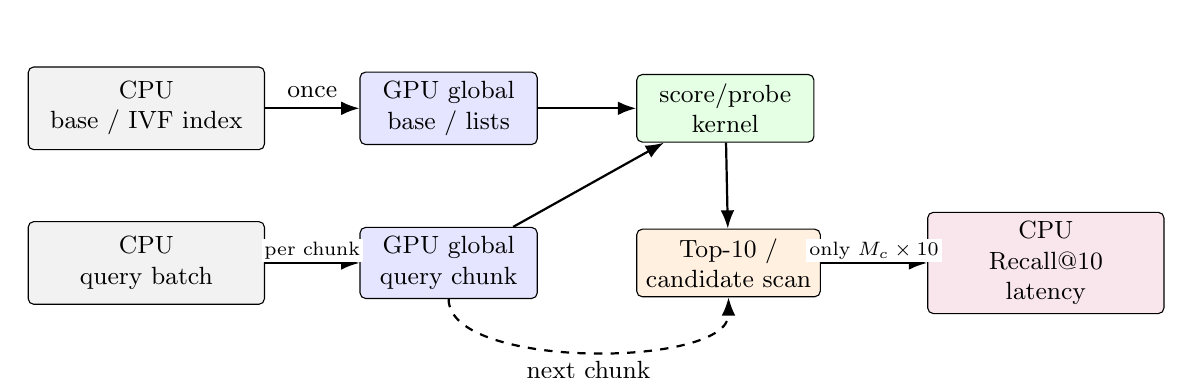
\begin{tikzpicture}[font=\small,>=Latex,node distance=1.1cm]
    \tikzset{
      box/.style={draw, rounded corners=2pt, align=center, minimum width=2.25cm, minimum height=0.82cm},
      big/.style={draw, rounded corners=2pt, align=center, minimum width=3.0cm, minimum height=1.05cm},
      arrow/.style={->, thick}
    }
    \node[big, fill=gray!10] (hostbase) {CPU\\base / IVF index};
    \node[big, fill=gray!10, below=0.9cm of hostbase] (hostquery) {CPU\\query batch};
    \node[box, fill=blue!10, right=1.2cm of hostbase] (devbase) {GPU global\\base / lists};
    \node[box, fill=blue!10, right=1.2cm of hostquery] (devquery) {GPU global\\query chunk};
    \node[box, fill=green!10, right=1.25cm of devbase] (score) {score/probe\\kernel};
    \node[box, fill=orange!12, right=1.25cm of devquery] (topk) {Top-$10$ /\\candidate scan};
    \node[big, fill=purple!10, right=1.35cm of topk] (result) {CPU\\Recall@10\\latency};
    \draw[arrow] (hostbase) -- node[above]{once} (devbase);
    \draw[arrow] (hostquery) -- node[above, midway, fill=white, inner sep=1pt, font=\scriptsize]{per chunk} (devquery);
    \draw[arrow] (devbase) -- (score);
    \draw[arrow] (devquery) -- (score);
    \draw[arrow] (score) -- (topk);
    \draw[arrow] (topk) -- node[above, midway, fill=white, inner sep=1pt, font=\scriptsize]
      {only $M_c\times10$} (result);
    \draw[arrow, dashed] (devquery.south) .. controls +(0,-0.9) and +(0,-0.9) ..
      node[below]{next chunk} (topk.south);
  \end{tikzpicture}
  \caption{CUDA batch ANN 搜索的数据流与任务划分}
  \label{fig:cuda_flow}
\end{figure}

在内存布局上，base 按 \code{base[base_id][dim]} 连续存储，query 按 \code{queries[query_id][dim]} 连续存储。score tile 则采用转置布局 \code{scores[query_id][base_id]}。这样做的原因是 Top-$k$ kernel 每个 block 处理一个 query，若该 query 的所有 base 得分连续，线程分片扫描时全局内存访问更规则，输出的 Top-$10$ 也可以直接写入 \code{out_dist[query][slot]} 和 \code{out_id[query][slot]}。

\subsection{GEMM score kernel}

\code{ScoreGemmKernel} 使用 $16\times16$ tile。block 的 $x$ 方向对应 base 行，$y$ 方向对应 query 行；每个线程负责一个 \code{(base_id, query_id)} 输出元素。kernel 在 $D$ 维上按 tile 遍历，将 base tile 和 query tile 载入共享内存，再在寄存器中累加内积。

\begin{lstlisting}[language=C++]
dim3 block(16, 16);
dim3 grid(DivUp(base_n, 16), DivUp(chunk, 16));
ScoreGemmKernel<<<grid, block>>>(d_base, d_queries, d_scores,
                                 static_cast<int>(base_n),
                                 static_cast<int>(chunk),
                                 static_cast<int>(dim));
\end{lstlisting}

该 kernel 对应的数学运算为
\[
\mathrm{score}_{q,b}=\sum_{t=0}^{D-1}B_{b,t}Q_{q,t}.
\]
由于 DEEP100K 的维度固定且远小于 base 数量，主要并行度来自 base 行和 query 行两个方向。共享内存 tile 减少了同一 block 内对 base/query 元素的重复读取；score 采用 query-major 存储则服务于下一步 Top-$k$。

为评估矩阵乘法优化空间，flat 路径加入 cuBLAS SGEMM 作为对照。实现中利用 \code{cublasSgemm} 计算同一批 query 与 base 的内积，并保持输出仍为 \code{scores[query][base]} 的 query-major 视图，后续 Top-$k$ kernel 不需要改变接口。该设计将手写 tiled kernel 与成熟 GEMM 库置于相同 Recall 和相同 Top-$k$ 后处理口径下，便于定量比较矩阵乘法优化效果。

\subsection{设备端 Top-k 合并}

Top-$k$ 是 ANN 搜索中容易被忽视的后处理瓶颈。如果将完整 score tile 拷回 CPU，再为每个 query 排序，会产生大量无意义的数据传输。本实现保留两个 Top-$k$ 版本用于对照。基础版 \code{ScoreTopKKernel} 每个 block 处理一个 query，block 内线程以 stride 方式扫描该 query 的所有 base 得分。每个线程在寄存器中维护自己的局部 Top-$10$，扫描结束后把局部候选写入共享内存，由线程 0 归并为最终 Top-$10$ 并按距离写出。优化版 \code{ScoreTopKTreeKernel} 仍先由各线程产生局部 Top-$10$，但 block 内候选合并改成共享内存树形归并，逐轮把参与线程数减半，减少末端单线程顺序比较。

\begin{lstlisting}[language=C++]
ScoreTopKKernel<<<static_cast<unsigned int>(chunk), threads,
                  shared_bytes>>>(d_scores, d_dist, d_ids,
                                  static_cast<int>(base_n));
ScoreTopKTreeKernel<<<static_cast<unsigned int>(chunk), threads,
                      shared_bytes>>>(d_scores, d_dist, d_ids,
                                      static_cast<int>(base_n));
\end{lstlisting}

该设计具有两个主要收益。第一，回传数据量从 $M_c\times N$ 个 float 降为 $M_c\times10$ 个距离和 id。第二，Top-$10$ 与 score tile 的生命周期绑定，GPU 完成 Top-$10$ 后该 chunk 的 score buffer 即可复用，不需要长期保存全局得分矩阵。由于 $k=10$ 很小，局部插入式维护 Top-$k$ 比完整排序更合适，也避免了引入复杂的全局排序依赖。

图 \ref{fig:topk_butterfly} 用蝶形归并的形式概括优化版 Top-$k$ 的信息流。实际实现中，每个线程先以 stride 方式扫描该 query 的若干 base 得分，并在寄存器中维护局部 Top-$10$；随后所有线程把局部候选写入共享内存。基础版由线程 0 对 \code{blockDim.x * 10} 个候选做一次顺序合并，优化版则让相邻线程的候选逐层合并，最后只留下线程 0 写出最终 Top-$10$。该实现仍不是完整排序，而是针对 $k=10$ 的选择问题减少候选规模和串行尾部。

\begin{figure}[H]
  \centering
  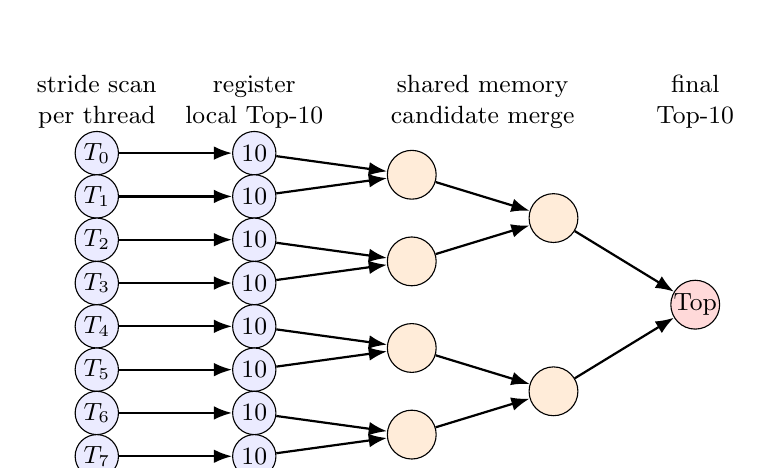
\begin{tikzpicture}[font=\small,>=Latex]
    \tikzset{
      node/.style={circle, draw, fill=blue!8, minimum size=0.55cm, inner sep=0pt},
      merge/.style={circle, draw, fill=orange!15, minimum size=0.62cm, inner sep=0pt},
      arrow/.style={->, thick}
    }
    \foreach \i in {0,...,7} {
      \node[node] (t\i) at (0,-0.55*\i) {$T_{\i}$};
      \node[node] (l\i) at (2.0,-0.55*\i) {$10$};
      \draw[arrow] (t\i) -- (l\i);
    }
    \foreach \i/\j/\y in {0/1/-0.275,2/3/-1.375,4/5/-2.475,6/7/-3.575} {
      \node[merge] (m\i) at (4.0,\y) {};
      \draw[arrow] (l\i) -- (m\i);
      \draw[arrow] (l\j) -- (m\i);
    }
    \foreach \a/\b/\y/\name in {0/2/-0.825/a,4/6/-3.025/b} {
      \node[merge] (n\name) at (5.8,\y) {};
      \draw[arrow] (m\a) -- (n\name);
      \draw[arrow] (m\b) -- (n\name);
    }
    \node[merge, fill=red!15] (out) at (7.6,-1.925) {Top};
    \draw[arrow] (na) -- (out);
    \draw[arrow] (nb) -- (out);
    \node[align=center] at (0,0.65) {stride scan\\per thread};
    \node[align=center] at (2.0,0.65) {register\\local Top-$10$};
    \node[align=center] at (4.9,0.65) {shared memory\\candidate merge};
    \node[align=center] at (7.6,0.65) {final\\Top-$10$};
  \end{tikzpicture}
  \caption{设备端 Top-$k$ 的局部候选压缩与蝶形归并示意}
  \label{fig:topk_butterfly}
\end{figure}

\subsection{IVF batch 搜索}

\code{ivf} 和 \code{ivf_grouped} 模式共同实现了作业提示中提到的 IVF 查询间并行。CPU 端先构建轻量 coarse quantizer：选择 $nlist$ 个初始 centroid，做少量 k-means 更新，将 base 向量分配到最近 centroid，并把每个 list 中的向量和原始 id 连续存放。per-query IVF 在线查询时，GPU 端执行三个阶段：
\begin{enumerate}
  \item \code{ScoreGemmKernel} 计算 query chunk 到所有 centroid 的内积得分；
  \item \code{SelectProbeKernel} 为每个 query 选择最近的 \code{nprobe} 个簇；
  \item \code{IvfSearchKernel} 只扫描这些候选簇中的向量，并在 block 内合并 Top-$10$。
\end{enumerate}

IVF 的一个难点是 batch 内不同 query 的最近簇编号通常不同。本实验保留 per-query probe list 作为基线：每个 query block 根据自己的 \code{nprobe} 列表扫描候选 list。该实现较为直接，但不同 query 的候选集合和 list 顺序不一致，候选扫描难以变成规则矩阵乘法。

为对照作业中提出的分组策略，\code{ivf_grouped} 模式在 probe selection 后按簇 id 对 batch 内 query 分桶。具体流程是：先把每个 query 的 \code{nprobe} 结果拷回主机侧；再为每个 list 收集需要探测该 list 的 query id，并把这些 query 打包成连续小矩阵；随后对同一个 list 的候选向量矩阵与该组 query 矩阵做一次 GEMM 式扫描；最后使用带全局 id 的 \code{ScoreTopKWithIdsTreeKernel} 产生每个 query 在该 list 内的局部 Top-$10$，并在主机端把同一 query 来自多个 probe list 的候选再合并成最终结果。该路径会增加分桶、重排和结果合并开销，但能够将“一个簇里的向量写成矩阵”的思路落实到 batch 计算流程中。

从搜索质量看，flat 模式是全量扫描，主要用于获得稳定的 Recall@10；IVF 模式通过 \code{nlist} 和 \code{nprobe} 控制候选规模，体现近似搜索中速度与召回率的折中。推荐的初始 IVF 配置为 16 个 coarse list、每个 query 探测 4 个 list，对应运行命令见第 \ref{sec:compile_run} 节。

\section{正确性与性能评估方法}

\subsection{编译与运行命令}
\label{sec:compile_run}

运行前先进入本次实验使用的环境：
\begin{lstlisting}[language=bash]
micromamba activate test
\end{lstlisting}

在 Linux 或已经配置 Visual Studio C++ host compiler 的 Windows CUDA 环境中，可以直接使用 Makefile。本机 Windows 环境已安装 Visual Studio Build Tools 到 \code{C:\BuildTools}，\code{Makefile} 会在 Windows 下自动调用 \code{vcvars64.bat} 加载 MSVC host compiler：
\begin{lstlisting}[language=bash]
cd ann-gpu
mingw32-make
.\build\main.exe gemm 2000
\end{lstlisting}

也可以绕过 Makefile 直接调用 \code{nvcc}。Windows PowerShell 下需先加载 VS Build Tools 环境：
\begin{lstlisting}[language=bash]
cmd /C "call C:\BuildTools\VC\Auxiliary\Build\vcvars64.bat && ^
        nvcc -O3 -x cu main.cc -o build\main.exe -lcublas"
.\build\main.exe ivf 2000 16 4
\end{lstlisting}

命令行参数含义为：\code{mode} 可取 \code{gemm}、\code{gemm_tree}、\code{cublas}、\code{cublas_tree}、\code{ivf} 或 \code{ivf_grouped}，省略时默认为 \code{gemm}；\code{query_n} 表示参与搜索的 query 数，默认 2000；\code{nlist} 和 \code{nprobe} 仅用于 IVF 模式，默认分别为 16 和 4。典型对照命令如下：

\begin{lstlisting}[language=bash]
.\build\main.exe cublas_tree 2000
.\build\main.exe ivf 2000 16 4
.\build\main.exe ivf_grouped 2000 16 4
\end{lstlisting}

\subsection{输出字段与评价含义}

程序输出示例如下：
\begin{lstlisting}[language=bash]
gpu_gemm_batch_topk, device="...", query_n=2000, base_n=100000, dim=96
average recall: ...
average latency (us): ...
wall latency including setup (us): ...
base/index copy or build (ms): ...
query copy (ms): ...
score/probe compute (ms): ...
topk/search compute (ms): ...
result copy (ms): ...
\end{lstlisting}

其中 \code{average recall} 是正确性指标；\code{average latency (us)} 由 CUDA event 统计在线阶段平均延迟；\code{wall latency including setup (us)} 包含主机端调用和一次性准备成本。其余字段用于拆分性能来源：base/index 首次拷贝或构建、query chunk 拷贝、score/probe kernel、Top-$10$/候选扫描 kernel 以及结果回传。

\subsection{本地工具链与重复测量结果}

本地机器配置为 NVIDIA GeForce RTX 4060 Laptop GPU、CUDA 12.4 和 Visual Studio Build Tools 2022。由于普通 PowerShell 中 \code{cl.exe} 不默认进入 \code{PATH}，本实验在 \code{Makefile} 中为 Windows 增加了 \code{C:\BuildTools\VC\Auxiliary\Build\vcvars64.bat} 的自动加载逻辑。执行 \code{mingw32-make clean} 和 \code{mingw32-make} 后，验证结果表明 \code{build/main.exe} 可正常生成。

为降低单次运行偶然波动的影响，表 \ref{tab:local_results} 和表 \ref{tab:ivf_grouped} 均采用同一机器上连续 3 次运行的均值与标准差，原始日志保存在 \path{report/results/gpu_variants_repeat_20260620.txt}，汇总文件为 \path{report/results/gpu_variants_repeat_20260620_summary.csv}。其中 \code{online/us} 是程序输出的在线阶段平均单 query 延迟，\code{wall/us} 是包含 setup 的端到端平均单 query 延迟；延迟与分段耗时列写作均值 $\pm$ 标准差，Recall@10 三次运行完全一致，因此表中只列均值。

\begin{table}[H]
  \centering\scriptsize
  \setlength{\tabcolsep}{3.0pt}
  \begin{tabularx}{\textwidth}{p{2.35cm}p{1.15cm}p{2.25cm}p{2.15cm}p{2.05cm}p{2.05cm}Y}
    \toprule
    模式 & 次数 & Recall@10 & online/us & wall/us & score ms & Top-$k$ ms \\
    \midrule
    \code{gemm} & 3 & 0.99990 & 237.63 $\pm$ 21.98 & 331.43 $\pm$ 19.30 & 240.08 $\pm$ 22.53 & 226.56 $\pm$ 17.40 \\
    \code{gemm_tree} & 3 & 0.99995 & 165.05 $\pm$ 11.33 & 256.43 $\pm$ 31.26 & 229.94 $\pm$ 14.38 & 91.92 $\pm$ 4.21 \\
    \code{cublas} & 3 & 0.99990 & 145.27 $\pm$ 1.10 & 233.59 $\pm$ 15.99 & 69.47 $\pm$ 1.34 & 214.49 $\pm$ 0.75 \\
    \code{cublas_tree} & 3 & 0.99995 & 83.24 $\pm$ 2.12 & 162.95 $\pm$ 6.73 & 70.71 $\pm$ 1.85 & 89.44 $\pm$ 2.41 \\
    \bottomrule
  \end{tabularx}
  \caption{Flat GEMM 路径的重复测量结果。数据集为 DEEP100K，\code{query_n=2000}，$k=10$。}
  \label{tab:local_results}
\end{table}

表 \ref{tab:local_results} 对“更快的矩阵乘法”和“更快的 Top-$k$”两项优化方向进行了对照。手写 tiled GEMM 的 score 阶段为 240.08 ms，而 cuBLAS SGEMM 为 69.47 ms；在相同数据规模下，cuBLAS 把矩阵乘法阶段缩短到约 $0.29\times$。Top-$k$ 方面，原始 \code{ScoreTopKKernel} 的末端由线程 0 顺序合并 \code{blockDim.x * 10} 个候选；优化后的 \code{ScoreTopKTreeKernel} 改用共享内存树形合并，使 Top-$k$ 阶段从 226.56 ms 降到 91.92 ms。两者叠加后，\code{cublas_tree} 的在线延迟降到 83.24 $\mu$s/query，是本实验中 Recall 接近 1 的最快 flat 配置。

\begin{table}[H]
  \centering\scriptsize
  \setlength{\tabcolsep}{3.0pt}
  \begin{tabularx}{\textwidth}{p{2.65cm}p{1.1cm}p{2.05cm}p{2.05cm}p{2.05cm}p{2.05cm}Y}
    \toprule
    模式 & nprobe & Recall@10 & online/us & wall/us & score/probe ms & search/Top-$k$ ms \\
    \midrule
    \code{ivf} & 2 & 0.87335 & 298.15 $\pm$ 35.46 & 494.82 $\pm$ 55.64 & 4.24 $\pm$ 2.92 & 582.22 $\pm$ 67.41 \\
    \code{ivf_grouped} & 2 & 0.87340 & 94.01 $\pm$ 10.35 & 277.34 $\pm$ 7.24 & 53.75 $\pm$ 3.24 & 53.02 $\pm$ 3.09 \\
    \code{ivf} & 4 & 0.96275 & 468.19 $\pm$ 34.50 & 688.25 $\pm$ 56.05 & 3.34 $\pm$ 0.34 & 922.68 $\pm$ 65.67 \\
    \code{ivf_grouped} & 4 & 0.96280 & 145.32 $\pm$ 38.71 & 375.75 $\pm$ 61.74 & 87.72 $\pm$ 5.84 & 64.04 $\pm$ 4.53 \\
    \code{ivf} & 8 & 0.99340 & 789.29 $\pm$ 89.28 & 987.22 $\pm$ 94.53 & 4.48 $\pm$ 1.76 & 1564.40 $\pm$ 172.34 \\
    \code{ivf_grouped} & 8 & 0.99345 & 189.90 $\pm$ 36.41 & 419.52 $\pm$ 65.88 & 143.18 $\pm$ 5.68 & 89.95 $\pm$ 4.06 \\
    \bottomrule
  \end{tabularx}
  \caption{IVF per-query probe list 与 grouped-IVF 的对照实验。两条路径使用相同的 $nlist=16$ 和相同的 \code{nprobe}。}
  \label{tab:ivf_grouped}
\end{table}

表 \ref{tab:ivf_grouped} 是针对作业中“让 batch 内最近簇编号重合度较高，避免计算资源浪费”的补充实验。per-query 路径中，每个 query block 直接扫描自己的 probe list，控制逻辑简单，但不同 query 的候选集合不一致，导致候选扫描 kernel 很难形成规则矩阵乘法形态。grouped-IVF 先在 GPU 上得到每个 query 的 \code{nprobe}，再按 probe 簇编号在主机侧分桶和重排；同一簇中的 query 被打包成一个小 batch，对该簇内向量矩阵执行一次 GEMM 式扫描，再用 \code{ScoreTopKWithIdsTreeKernel} 产生带全局 id 的局部 Top-$10$，最后在主机端按 query 合并各 probe 簇的结果。

实验结果显示，在相同 \code{nprobe} 下 grouped-IVF 的 Recall 与 per-query 基本一致，但在线延迟明显降低。以 \code{nprobe=4} 为例，per-query 的在线延迟为 468.19 $\mu$s/query，grouped-IVF 为 145.32 $\mu$s/query，约为前者的 $0.31\times$；搜索/Top-$k$ 阶段也从 922.68 ms 降到 64.04 ms。grouped-IVF 的代价是额外的 query 分桶、重排、结果拷贝和主机端合并，因此 \code{score/probe ms} 与 \code{result copy ms} 上升；但候选扫描变成更规则的批量矩阵乘法后，总体仍然更快。结果表明，分组策略是 IVF 在 GPU batch 场景中的重要优化点；后续仍可进一步将分桶与最终合并迁移至 GPU 端，以减少主机参与。

\subsection{与 CPU 基线的加速比}

为保持与前序 ANN 实验相同的评价口径，表 \ref{tab:gpu_speedup} 给出 GPU 实现相对 CPU Flat 基线的加速比。CPU 基线来自同一份 DEEP100K、\code{query_n=2000}、$k=10$ 的 Windows i9-13900H SIMD 实验：串行 Flat 为 4571.62 $\mu$s/query，Flat-AVX2 为 1756.11 $\mu$s/query，二者 Recall@10 均为 0.99995。表中 \code{online} 加速比使用 GPU 输出的 \code{average latency (us)} 作为分母，表示 base/index 已准备好之后的在线查询吞吐；\code{wall} 加速比使用 \code{wall latency including setup (us)}，把一次性 base 拷贝或 IVF 构建也计入分母。

\begin{table}[H]
  \centering\scriptsize
  \setlength{\tabcolsep}{3.0pt}
  \begin{tabular}{lrrrrrrr}
    \toprule
    GPU 配置 & Recall@10 & online/us & wall/us & online vs 串行 & online vs AVX2 & wall vs 串行 & wall vs AVX2 \\
    \midrule
    \code{gemm} & 0.99990 & 237.63 & 331.43 & 19.24$\times$ & 7.39$\times$ & 13.79$\times$ & 5.30$\times$ \\
    \code{cublas_tree} & 0.99995 & 83.24 & 162.95 & 54.92$\times$ & 21.10$\times$ & 28.05$\times$ & 10.78$\times$ \\
    \code{ivf_grouped}/4 & 0.96280 & 145.32 & 375.75 & 31.46$\times$ & 12.08$\times$ & 12.17$\times$ & 4.67$\times$ \\
    \code{ivf_grouped}/8 & 0.99345 & 189.90 & 419.52 & 24.07$\times$ & 9.25$\times$ & 10.90$\times$ & 4.19$\times$ \\
    \bottomrule
  \end{tabular}
  \caption{GPU 实现相对 CPU Flat 基线的加速比。CPU 基线来自前序 SIMD 实验结果文件；GPU 数值使用 3 次重复测量均值。}
  \label{tab:gpu_speedup}
\end{table}

加速比需结合 Recall 共同解释。\code{cublas_tree} 是最可比的一行：它和 CPU Flat 都是全量扫描，Recall 接近 1，在线阶段相对串行 Flat 达到 $54.92\times$，即使计入一次性 setup 仍有 $28.05\times$。\code{ivf_grouped}/8 在 Recall@10 = 0.99345 时在线延迟为 189.90 $\mu$s/query，相比串行 Flat 仍有 $24.07\times$ 加速；\code{ivf_grouped}/4 则体现更激进的速度/召回取舍。因此，评价 GPU 配置时需要同时给出 Recall、latency、setup 口径和相对基线。

\begin{figure}[H]
  \centering
  \begin{tikzpicture}[font=\small,>=Latex]
    \draw[->] (0,0) -- (8.8,0) node[right, font=\scriptsize]{配置};
    \draw[->] (0,0) -- (0,5.35);
    \node[font=\scriptsize, rotate=90, anchor=south] at (-0.72,2.75) {在线延迟 / $\mu\mathrm{s}$};
    \node[font=\scriptsize, anchor=east] at (8.2,5.25) {柱顶标注 Recall@10};
    \foreach \y/\tick in {0/0,1/50,2/100,3/150,4/200,5/250} {
      \draw[gray!30] (0,\y) -- (8.0,\y);
      \node[left, font=\scriptsize] at (0,\y) {\tick};
    }
    \foreach \x/\h/\name/\lat/\rec/\color in {
      1.15/4.753/GEMM/237.63/0.9999/blue!45,
      3.25/1.665/cuBLAS-tree/83.24/0.99995/blue!70,
      5.35/2.906/IVF-g4/145.32/0.9628/orange!65,
      7.35/3.798/IVF-g8/189.90/0.99345/orange!85} {
      \draw[fill=\color, draw=black!35] (\x-0.42,0) rectangle (\x+0.42,\h);
      \node[below, font=\scriptsize, align=center] at (\x,-0.10) {\name};
      \node[above, align=center, font=\tiny, fill=white, inner sep=0.8pt, yshift=1pt] at (\x,\h)
        {\lat\\Recall \rec};
    }
  \end{tikzpicture}
  \caption{代表性 GPU 配置的在线延迟与 Recall@10，数据为 3 次重复测量均值}
  \label{fig:gpu_latency_recall}
\end{figure}

\begin{figure}[H]
  \centering
  \begin{tikzpicture}[font=\small]
    \draw[->] (0,0) -- (8.8,0);
    \node[above] at (4.35,4.55) {累计 CUDA event 耗时 / ms};
    \foreach \x/\label in {0/0,2/200,4/400,6/600,8/800} {
      \draw[gray!30] (\x,0) -- (\x,4.10);
      \node[below, font=\scriptsize] at (\x,0) {\label};
    }
    \foreach \y/\name in {3.65/GEMM,2.80/cuBLAS-tree,1.95/IVF-g4,1.10/IVF-g8} {
      \node[left, font=\scriptsize, align=right] at (0,\y+0.15) {\name};
    }
    % scale: 100 ms = 1 tikz unit.
    \def\barh{0.30}
    \foreach \y/\q/\s/\t/\r in {
      3.65/0.019/2.401/2.266/0.067,
      2.80/0.011/0.707/0.894/0.052,
      1.95/0.292/0.877/0.640/0.847,
      1.10/0.306/1.432/0.900/0.892} {
      \draw[fill=teal!55, draw=none] (0,\y) rectangle ++(\q,\barh);
      \draw[fill=blue!55, draw=none] (\q,\y) rectangle ++(\s,\barh);
      \draw[fill=orange!70, draw=none] (\q+\s,\y) rectangle ++(\t,\barh);
      \draw[fill=purple!55, draw=none] (\q+\s+\t,\y) rectangle ++(\r,\barh);
    }
    \foreach \x/\y/\label in {4.82/3.81/475.3,1.75/2.96/166.5,2.75/2.11/265.7,3.62/1.26/352.9} {
      \node[right, font=\scriptsize] at (\x,\y) {\label};
    }
    \node[fill=teal!55, minimum width=0.32cm, minimum height=0.16cm] at (0.75,-0.68) {};
    \node[right, font=\scriptsize] at (0.93,-0.68) {query copy};
    \node[fill=blue!55, minimum width=0.32cm, minimum height=0.16cm] at (2.65,-0.68) {};
    \node[right, font=\scriptsize] at (2.83,-0.68) {score/probe};
    \node[fill=orange!70, minimum width=0.32cm, minimum height=0.16cm] at (4.80,-0.68) {};
    \node[right, font=\scriptsize] at (4.98,-0.68) {Top-$k$/search};
    \node[fill=purple!55, minimum width=0.32cm, minimum height=0.16cm] at (7.00,-0.68) {};
    \node[right, font=\scriptsize] at (7.18,-0.68) {result copy};
    \node[font=\scriptsize, anchor=east] at (8.65,4.12) {条末数字为总耗时};
  \end{tikzpicture}
  \caption{在线阶段 CUDA event 分段耗时，比例尺为 1 单位对应 100 ms}
  \label{fig:gpu_event_breakdown}
\end{figure}

表 \ref{tab:derived_perf} 进一步根据重复运行日志推导各阶段的有效吞吐。GEMM score 阶段的工作量按 $2NMD$ 次浮点操作估算；Top-$k$ 阶段按扫描得分个数估算；IVF 搜索阶段用于比较 per-query 与 grouped 两种候选扫描组织方式。该表不表示硬件峰值，只用于解释本实现中不同 kernel 的瓶颈差异。

\begin{table}[H]
  \centering\footnotesize
  \begin{tabularx}{\textwidth}{p{2.6cm}p{2.35cm}p{2.55cm}p{2.35cm}Y}
    \toprule
    阶段 & 有效工作量 & 对应耗时 & 派生指标 & 结论 \\
    \midrule
    手写 GEMM score & 38.4 GFLOP & 240.08 ms & 160.0 GFLOP/s & $16\times16$ tiled kernel 结构清晰，但距离 cuBLAS 仍有明显差距。\\
    cuBLAS score & 38.4 GFLOP & 69.47 ms & 552.7 GFLOP/s & 说明矩阵乘法阶段可以通过成熟库获得直接收益。\\
    线程 0 Top-$k$ & 2.0 亿个 score & 226.56 ms & 0.88 Gscore/s & 顺序合并候选成为和 score 同量级的瓶颈。\\
    树形 Top-$k$ & 2.0 亿个 score & 91.92 ms & 2.18 Gscore/s & 共享内存树形合并降低了 block 末端串行部分。\\
    IVF-4 per-query search & 约 5000 万候选 & 922.68 ms & 52.0 GFLOP/s & 候选 list 随 query 分散，kernel 形态不规则。\\
    IVF-4 grouped search & 约 5000 万候选 & 64.04 ms & 749.6 GFLOP/s & 按簇分桶后能以小批量 GEMM 扫描同一 list，显著改善候选阶段。\\
    \bottomrule
  \end{tabularx}
  \caption{由重复运行日志推导的 GPU 阶段吞吐与组织方式对比}
  \label{tab:derived_perf}
\end{table}

上述结果表明，GEMM 和 IVF 的差异不仅在于“全量扫描”与“近似候选扫描”。GEMM 的 score 阶段访存和计算形态规则，可以通过共享内存 tile 或 cuBLAS 获得稳定复用；Top-$k$ 的候选合并同样会成为全量扫描的主要瓶颈。IVF 的候选 list 则随 query 的 probe 结果变化，list 长度和访问位置都不完全一致；当按 list 分桶后，同一个簇内的向量矩阵可以被多个 query 共享扫描，虽然多了重排和合并开销，但能显著减少不规则 per-query 扫描带来的浪费。

\section{实验分析}

\subsection{GEMM 路径分析}

\code{gemm} 模式的主要计算量为 $O(NM_cD)$。在 DEEP100K 中，$N$ 远大于 $D$，因此 kernel 的并行度主要来自 base 行方向；batch query 又在另一个维度提供并行度。与单 query 相比，batch 方式可以把 base 常驻显存，并让同一份 base tile 被多个 query 输出复用。

显存占用由四部分构成：base 常驻数组、query chunk、score tile 和 Top-$10$ 输出。score tile 是最大临时数组，因此 chunk 大小需要在并行度和显存占用之间折中。本实现默认 \code{query_chunk=128}，此时 score tile 大小约为 $128\times100000\times4\approx48.8$ MiB，既能提供足够 query 并行度，又不会接近常见消费级 GPU 显存上限。实验结果表明，手写 tiled GEMM 更适合作为 CUDA tile 设计的说明性实现；cuBLAS 更适合作为高性能基线。二者共用同一 Top-$k$ 后处理，有助于区分 score 计算和候选选择两个瓶颈。

\subsection{Top-k 路径分析}

Top-$k$ kernel 的扫描复杂度为 $O(M_cN)$，但其输出规模只有 $O(M_ck)$。由于 $k=10$ 固定且较小，线程局部数组可以放在寄存器中维护；block 内合并时共享内存占用为
\[
\mathrm{threads}\times k\times(\mathrm{sizeof(float)}+\mathrm{sizeof(uint32\_t)}).
\]
\code{ClampThreads} 会根据设备共享内存限制裁剪线程数，避免动态共享内存超过单 block 限制。该设计比完整排序更符合 ANN Top-$k$ 场景：只保留前 10 个候选，既减少计算，也减少回传。基础版 Top-$k$ 暴露出线程 0 顺序合并的瓶颈，树形合并版则用更多线程参与 block 内候选归并，使 Top-$k$ 阶段耗时降低到基础版的约 $0.41\times$。

\subsection{IVF 路径分析}

IVF 模式的在线开销可分为 centroid scoring、probe selection、candidate search 和最终 Top-$k$ 合并。centroid 数量 $nlist$ 通常远小于 base 数量，因此 per-query 基线中第一阶段开销较小；第二阶段开销取决于 \code{nprobe} 个 list 的总长度。若 \code{nprobe} 增大，召回率通常上升，但候选扫描时间也增加；若 \code{nprobe} 过小，搜索速度提升，但容易漏掉真实近邻所在簇。

per-query 路径的优点是实现简单，每个 query block 直接读取自己的 probe list；缺点是不同 query 的候选集合不一致，GPU 上的访存和控制流更不规则。grouped-IVF 则把 batch 内 query 按 probe 簇编号重新分组，使同一个 list 的候选向量能够写成矩阵并被一组 query 共同扫描。表 \ref{tab:ivf_grouped} 显示，grouped-IVF 在相同 \code{nprobe} 下几乎不改变 Recall，却显著降低候选扫描时间。由此可见，作业提示中的分组策略并非单纯的工程性重排，而是能改变候选扫描 kernel 形态的关键设计。

\subsection{数据传输与设备端计算}

本实验把计时字段拆成 copy、score/probe、topk/search 和 result copy。该拆分用于判断瓶颈属于数据传输还是 kernel 计算。如果 \code{query copy} 和 \code{result copy} 占比较高，通常表明 batch 太小或传输开销未被计算充分覆盖；如果 \code{score/probe compute} 占比高，则表明 GEMM、cuBLAS 或 grouped-IVF 的分组扫描成为主瓶颈；如果 \code{topk/search compute} 占比高，则应重点检查 Top-$k$ 合并或 IVF 候选列表长度。表 \ref{tab:local_results} 中，基础 GEMM 的 score 和 Top-$k$ 都不可忽略；表 \ref{tab:ivf_grouped} 中，per-query IVF 的主要设备端耗时在候选 list 扫描，而 grouped-IVF 把该部分显著压缩，但会增加分桶、query/result 拷贝和主机合并开销。

加速比结果还反映出 setup 口径的重要性。GEMM 的 online 加速比高于 wall 加速比，是因为 base 首次拷贝、cuBLAS handle、结果缓冲分配和主机端调度在单次运行中不可忽略；IVF 的差距更明显，因为构建 coarse list 和倒排表需要额外准备时间。若实际系统连续处理多个 query batch，base 或 IVF index 可以常驻显存，online 口径更能反映吞吐；若只运行一次命令行程序，wall 口径更保守。

\subsection{静态 profile 与汇编分析}

本机 CUDA Toolkit 未安装 \code{nsys} 和 \code{ncu} 命令行工具，因此本节使用三类可复现证据进行性能剖析：第一，正文输出的 CUDA event 分段计时；第二，\code{cuobjdump --dump-resource-usage build/main.exe} 导出的 kernel 静态资源；第三，\code{nvcc --ptx} 与 \code{cuobjdump --dump-sass} 导出的 PTX/SASS 指令片段。云端环境虽可使用 Nsight Systems，但本次实验未在同一代码与数据路径下重新运行云端 timeline，因此本文未将 nsys 图作为定量分析依据。资源占用汇总见表 \ref{tab:cuda_resource}。

\begin{table}[H]
  \centering\footnotesize
  \begin{tabularx}{\textwidth}{p{3.6cm}rrrrY}
    \toprule
    Kernel & Reg & Stack/B & Static shared/B & Local/B & 含义 \\
    \midrule
    \code{ScoreGemmKernel} & 27 & 0 & 2048 & 0 & 两个 $16\times16$ float tile，各 1024 B；静态 shared memory 与源码 tile 设计一致。\\
    \code{ScoreTopKKernel} & 32 & 80 & 0 & 0 & 基础 Top-$k$ 保留线程局部数组，仍有少量栈用量。\\
    \code{ScoreTopKTreeKernel} & 32 & 0 & 0 & 0 & 树形合并版消除了静态栈用量，动态共享内存由 launch 时传入。\\
    \begin{tabular}[t]{@{}l@{}}\code{ScoreTopKWithIds}\\\code{TreeKernel}\end{tabular} & 32 & 0 & 0 & 0 & grouped-IVF 使用的带全局 id Top-$k$，资源形态与树形合并版接近。\\
    \code{IvfSearchKernel} & 31 & 160 & 0 & 0 & per-query IVF 每线程维护局部 Top-$10$，同时扫描候选 list，栈用量高于 GEMM。\\
    \code{SelectProbeKernel} & 32 & 256 & 0 & 0 & 单线程选择 \code{nprobe}，数组上限 32，开销小但并行度有限。\\
    \bottomrule
  \end{tabularx}
  \caption{CUDA kernel 静态资源占用，来源于 \code{cuobjdump_resource.txt}}
  \label{tab:cuda_resource}
\end{table}

PTX 输出中，\code{ScoreGemmKernel} 明确包含两个静态共享内存数组：
\begin{lstlisting}[language=bash]
.shared .align 4 .b8 base_tile[1024];
.shared .align 4 .b8 query_tile[1024];
ld.global.nc.f32 ...      // base/query global load
st.shared.f32 ...         // write tile into shared memory
bar.sync 0;
ld.shared.f32 ...
fma.rn.f32 ...
bar.sync 0;
\end{lstlisting}
该片段与源码中的 $16\times16$ tiled GEMM 一致。每轮 tile 先从全局内存读入 base 和 query，再写入共享内存；\code{bar.sync} 对应 \code{__syncthreads()}，保证 tile 完整后再执行 16 次 FMA 累加。SASS 中同一位置可见 \code{LDG}、\code{STS}、\code{LDS}、\code{FFMA} 与 \code{BAR.SYNC} 指令，说明编译器将内层乘加转成 fused multiply-add，并使用共享内存作为片上复用缓冲。对应的 SASS 片段如下，\code{STS} 将全局加载后的数据写入共享内存，\code{BAR.SYNC} 对应 tile 装载后的块内同步，\code{LDS} 从共享内存读取 tile 数据，\code{FFMA} 执行乘加累积：
\begin{lstlisting}[language=bash]
/*0310*/ STS [R22], R27;
/*0320*/ STS [R22+0x400], R29;
/*0330*/ BAR.SYNC.DEFER_BLOCKING 0x0;
/*0340*/ LDS R8, [R21];
/*03f0*/ FFMA R12, R12, R8, R9;
/*0580*/ BAR.SYNC.DEFER_BLOCKING 0x0;
\end{lstlisting}

\code{ScoreTopKKernel} 的 PTX/SASS 则呈现另一种形态：扫描阶段包含连续 \code{ld.global.nc.f32}，随后将每线程的 10 个候选写入动态共享内存。基础版末端由线程 0 读取共享内存并完成最终排序；树形版把候选合并拆成多轮共享内存归并，因此资源表中 \code{ScoreTopKTreeKernel} 的静态栈用量降为 0。结合图 \ref{fig:gpu_event_breakdown} 和表 \ref{tab:derived_perf}，全量扫描不仅受矩阵乘法约束，Top-$10$ 后处理也已经成为同量级开销。

IVF profile 结果更集中地反映候选组织方式的影响：per-query 路径中 \code{topk/search} 随 \code{nprobe} 增大快速上升，\code{nprobe=4} 时达到 922.68 ms；grouped-IVF 在相同 \code{nprobe=4} 下把该阶段降到 64.04 ms，但 \code{score/probe}、query copy 和 result copy 字段增加，反映出分桶、重排和主机端合并的额外代价。该现象表明，当前 IVF 在线阶段的主要矛盾不是 centroid 数量，而是候选 list 如何组织成适合 GPU 的规则批量计算。

\section{总结}

任务一 HIP 云学习系统梳理了 GPU 编程的共性方法：访存合并决定带宽型 kernel 的上限，共享内存适合做片上复用和重排，两级归约可以显著减少全局原子，warp/wave 内原语能够降低同步开销，多 kernel 编排则适合 K-Means 这类阶段性算法。

任务二 ANN GPU 实现完成了多条 GPU 搜索与对照路径。Flat 路径严格对应作业要求中的 batch 矩阵乘法，并进一步比较了手写 tiled GEMM、cuBLAS SGEMM、基础 Top-$k$ 和树形 Top-$k$；IVF 路径在 per-query probe list 基线之外，实现了按 probe 簇分桶的 grouped-IVF，对同一簇内向量矩阵与 query 小 batch 做 GEMM 式扫描。实测结果表明，\code{cublas_tree} 在 Recall@10 接近 1 时达到 83.24 $\mu$s/query；grouped-IVF 在 \code{nprobe=4} 时以 Recall@10 = 0.96280 换取 145.32 $\mu$s/query，在 \code{nprobe=8} 时以 189.90 $\mu$s/query 达到 Recall@10 = 0.99345。CUDA event、重复测量、cuobjdump 资源占用与 PTX/SASS 片段共同表明：ANN GPU 优化除距离计算外，还受到 Top-$k$ 合并和 IVF 候选组织方式的制约。

\clearpage
\section*{参考文献}
\addcontentsline{toc}{section}{参考文献}

\begin{enumerate}[label={[\arabic*]}]
  \item NVIDIA Corporation. \emph{CUDA C++ Programming Guide}. \url{https://docs.nvidia.com/cuda/cuda-c-programming-guide/}.
  \item NVIDIA Corporation. \emph{CUDA C++ Best Practices Guide}. \url{https://docs.nvidia.com/cuda/cuda-c-best-practices-guide/}.
  \item AMD ROCm Documentation. \emph{Introduction to the HIP Programming Model}. \url{https://rocm.docs.amd.com/projects/HIP/en/latest/understand/programming_model.html}.
  \item Jeff Johnson, Matthijs Douze, and Hervé Jégou. Billion-scale similarity search with GPUs. \emph{IEEE Transactions on Big Data}, 7(3):535--547, 2021. arXiv:1702.08734. \url{https://arxiv.org/abs/1702.08734}.
  \item Hervé Jégou, Matthijs Douze, and Cordelia Schmid. Product quantization for nearest neighbor search. \emph{IEEE Transactions on Pattern Analysis and Machine Intelligence}, 33(1):117--128, 2011. doi:10.1109/TPAMI.2010.57.
  \item Artem Babenko and Victor Lempitsky. Efficient indexing of billion-scale datasets of deep descriptors. In \emph{Proceedings of the IEEE Conference on Computer Vision and Pattern Recognition (CVPR)}, pages 2055--2063, 2016. \url{https://openaccess.thecvf.com/content_cvpr_2016/html/Babenko_Efficient_Indexing_of_CVPR_2016_paper.html}.
  \item 并行程序设计课程 GPU 编程作业要求、AMD AUP HIP Lab1--Lab6 notebook 与课程 ANN 实验框架。
  \item 本仓库前序 ANN SIMD 实验结果目录 \path{ann-SIMD/bench_results/windows_i9_13900h/} 中的 \path{baseline_flat.csv} 与 \path{RESULTS.md}。
\end{enumerate}

\clearpage
\appendix
\section{学习通过截图}
\label{app:screenshots}

本附录给出 AMD AUP 平台六个 Lab 的学习通过截图。部分原图为终端横向长截图，直接按整图缩放会导致文字偏小；因此，\code{report/fig/} 中放置关键输出区域的放大图，完整原始截图保存在 \code{ann-gpu/img/} 目录中。

\begin{figure}[H]
  \centering
  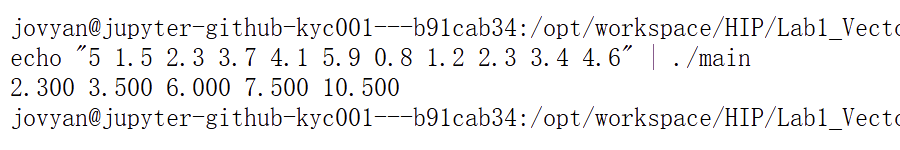
\includegraphics[width=\textwidth,height=0.22\textheight,keepaspectratio]{fig/lab1_zoom.png}
  \caption{Lab1 Vector Addition 学习通过截图关键区域}
  \label{fig:lab1}
\end{figure}

\begin{figure}[H]
  \centering
  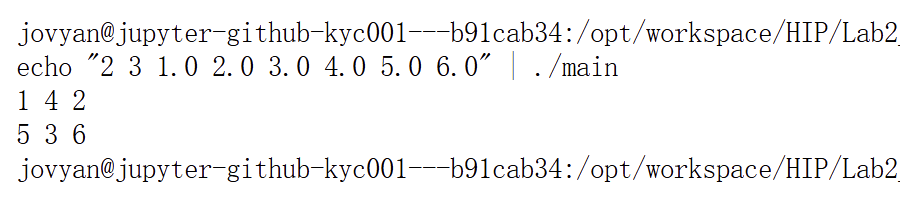
\includegraphics[width=\textwidth,height=0.28\textheight,keepaspectratio]{fig/lab2_zoom.png}
  \caption{Lab2 Matrix Transpose 学习通过截图关键区域}
  \label{fig:lab2}
\end{figure}

\clearpage
\begin{figure}[H]
  \centering
  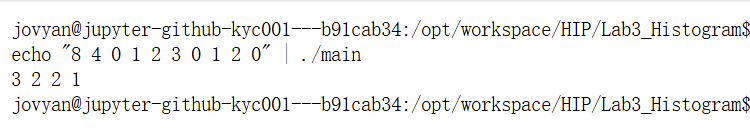
\includegraphics[width=\textwidth,height=0.22\textheight,keepaspectratio]{fig/lab3_zoom.png}
  \caption{Lab3 Histogram 学习通过截图关键区域}
  \label{fig:lab3}
\end{figure}

\begin{figure}[H]
  \centering
  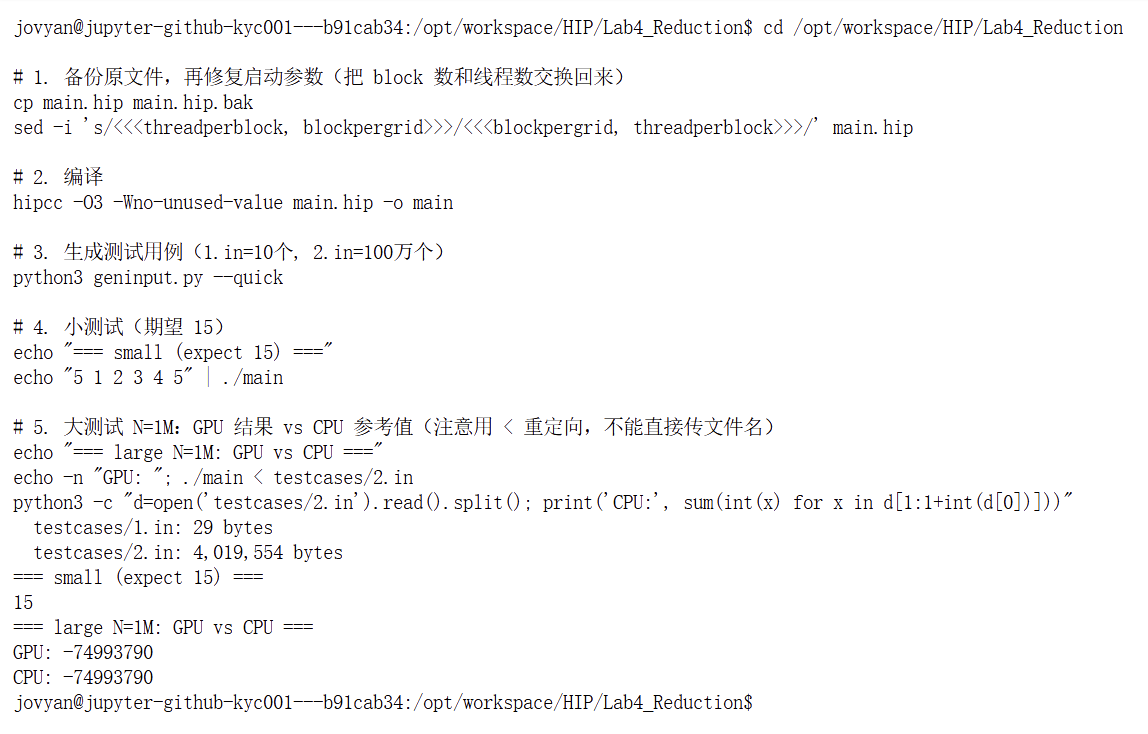
\includegraphics[width=\textwidth,height=0.55\textheight,keepaspectratio]{lab4.jpg}
  \caption{Lab4 Reduction 学习通过截图}
  \label{fig:lab4}
\end{figure}

\clearpage
\begin{figure}[H]
  \centering
  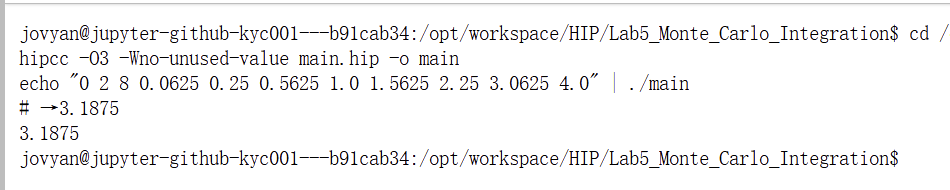
\includegraphics[width=\textwidth,height=0.28\textheight,keepaspectratio]{fig/lab5_zoom.png}
  \caption{Lab5 Monte Carlo 学习通过截图关键区域}
  \label{fig:lab5}
\end{figure}

\begin{figure}[H]
  \centering
  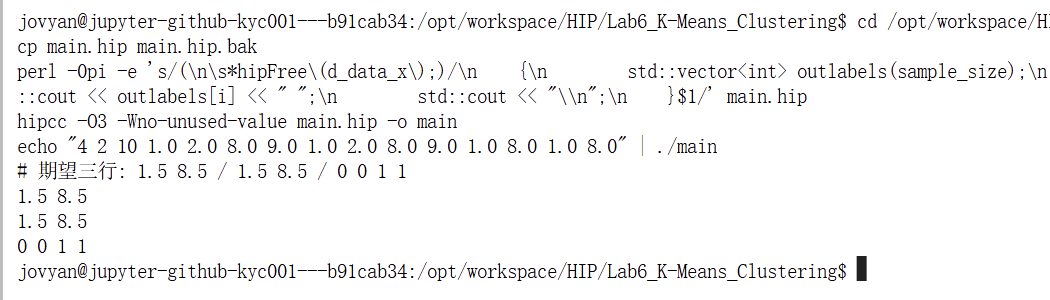
\includegraphics[width=\textwidth,height=0.40\textheight,keepaspectratio]{fig/lab6_zoom.png}
  \caption{Lab6 K-Means 学习通过截图关键区域}
  \label{fig:lab6}
\end{figure}

\clearpage
\section{AI 使用报告}
\label{app:ai}

实验过程中，生成式 AI 仅用于作业要求梳理、实现路线比较、代码结构检查和文字表达调整。实验数据、运行结果和性能结论均来自课程材料、本地编译运行与程序输出；可复现入口以 \code{main.cc}、\code{Makefile} 和正文列出的命令为准。

\begin{table}[H]
  \centering\footnotesize
  \begin{tabularx}{\textwidth}{p{3.1cm}Y Y}
    \toprule
    使用场景 & 使用目的 & 采用情况 \\
    \midrule
    作业范围确认 &
    明确 HIP 在线学习、ANN GPU 加速以及页数限制之间的关系。 &
    报告划分为两个独立任务；HIP 填空和截图作为基础要求材料，ANN 主体按进阶选题研究报告组织。 \\
    \midrule
    ANN GPU 路线 &
    比较单 query 与 batch query 的 GPU 实现方式，并评估完整 score 矩阵回传的必要性。 &
    采用 batch GEMM 与设备端 Top-$10$ 合并，减少主机端排序和完整得分矩阵回传。 \\
    \midrule
    工程结构与模块化 &
    保持 \code{main.cc} 框架尽量不改，并采用前几次实验的 header-only 风格。 &
    保留主程序薄入口，将 CUDA 公共工具、GEMM kernel、Top-$k$ kernel、GEMM 搜索和 IVF 搜索拆分到 \code{gpu/} 目录，由 \code{gpu_ann_search.cuh} 统一聚合。 \\
    \midrule
    性能分析取舍 &
    确定本次 ANN GPU 选题的性能分析范围。 &
    保留 CUDA event 分段计时和 correctness 验证，正文围绕数据传输、score/probe kernel 和 Top-$k$/search kernel 展开分析。 \\
    \midrule
    本地工具链问题 &
    定位 Windows 下 \code{nvcc} 编译失败的原因并完成本地验证。 &
    确认失败原因是缺少 \code{cl.exe} host compiler；随后补齐 Visual Studio Build Tools 到 \code{C:\BuildTools}，修改 \code{Makefile} 自动加载 \code{vcvars64.bat}，并完成 \code{gemm 2000} 与 \code{ivf 2000 16 4} 的本地运行验证。 \\
    \bottomrule
  \end{tabularx}
  \caption{生成式 AI 辅助使用记录}
  \label{tab:ai_usage}
\end{table}

\end{document}
